\documentclass[twoside]{book}

% Packages required by doxygen
\usepackage{calc}
\usepackage{doxygen}
\usepackage{graphicx}
\usepackage[utf8]{inputenc}
\usepackage{makeidx}
\usepackage{multicol}
\usepackage{multirow}
\usepackage{textcomp}
\usepackage[table]{xcolor}

% Font selection
\usepackage[T1]{fontenc}
\usepackage{mathptmx}
\usepackage[scaled=.90]{helvet}
\usepackage{courier}
\usepackage{amssymb}
\usepackage{sectsty}
\renewcommand{\familydefault}{\sfdefault}
\allsectionsfont{%
  \fontseries{bc}\selectfont%
  \color{darkgray}%
}
\renewcommand{\DoxyLabelFont}{%
  \fontseries{bc}\selectfont%
  \color{darkgray}%
}

% Page & text layout
\usepackage{geometry}
\geometry{%
  a4paper,%
  top=2.5cm,%
  bottom=2.5cm,%
  left=2.5cm,%
  right=2.5cm%
}
\tolerance=750
\hfuzz=15pt
\hbadness=750
\setlength{\emergencystretch}{15pt}
\setlength{\parindent}{0cm}
\setlength{\parskip}{0.2cm}
\makeatletter
\renewcommand{\paragraph}{%
  \@startsection{paragraph}{4}{0ex}{-1.0ex}{1.0ex}{%
    \normalfont\normalsize\bfseries\SS@parafont%
  }%
}
\renewcommand{\subparagraph}{%
  \@startsection{subparagraph}{5}{0ex}{-1.0ex}{1.0ex}{%
    \normalfont\normalsize\bfseries\SS@subparafont%
  }%
}
\makeatother

% Headers & footers
\usepackage{fancyhdr}
\pagestyle{fancyplain}
\fancyhead[LE]{\fancyplain{}{\bfseries\thepage}}
\fancyhead[CE]{\fancyplain{}{}}
\fancyhead[RE]{\fancyplain{}{\bfseries\leftmark}}
\fancyhead[LO]{\fancyplain{}{\bfseries\rightmark}}
\fancyhead[CO]{\fancyplain{}{}}
\fancyhead[RO]{\fancyplain{}{\bfseries\thepage}}
\fancyfoot[LE]{\fancyplain{}{}}
\fancyfoot[CE]{\fancyplain{}{}}
\fancyfoot[RE]{\fancyplain{}{\bfseries\scriptsize Generated on Fri Aug 29 2014 12\-:13\-:17 for Web Page Comparator by Doxygen }}
\fancyfoot[LO]{\fancyplain{}{\bfseries\scriptsize Generated on Fri Aug 29 2014 12\-:13\-:17 for Web Page Comparator by Doxygen }}
\fancyfoot[CO]{\fancyplain{}{}}
\fancyfoot[RO]{\fancyplain{}{}}
\renewcommand{\footrulewidth}{0.4pt}
\renewcommand{\chaptermark}[1]{%
  \markboth{#1}{}%
}
\renewcommand{\sectionmark}[1]{%
  \markright{\thesection\ #1}%
}

% Indices & bibliography
\usepackage{natbib}
\usepackage[titles]{tocloft}
\setcounter{tocdepth}{3}
\setcounter{secnumdepth}{5}
\makeindex

% Hyperlinks (required, but should be loaded last)
\usepackage{ifpdf}
\ifpdf
  \usepackage[pdftex,pagebackref=true]{hyperref}
\else
  \usepackage[ps2pdf,pagebackref=true]{hyperref}
\fi
\hypersetup{%
  colorlinks=true,%
  linkcolor=blue,%
  citecolor=blue,%
  unicode%
}

% Custom commands
\newcommand{\clearemptydoublepage}{%
  \newpage{\pagestyle{empty}\cleardoublepage}%
}


%===== C O N T E N T S =====

\begin{document}

% Titlepage & ToC
\hypersetup{pageanchor=false}
\pagenumbering{roman}
\begin{titlepage}
\vspace*{7cm}
\begin{center}%
{\Large Web Page Comparator \\[1ex]\large 1.\-0.\-5 }\\
\vspace*{1cm}
{\large Generated by Doxygen 1.8.6}\\
\vspace*{0.5cm}
{\small Fri Aug 29 2014 12:13:17}\\
\end{center}
\end{titlepage}
\clearemptydoublepage
\tableofcontents
\clearemptydoublepage
\pagenumbering{arabic}
\hypersetup{pageanchor=true}

%--- Begin generated contents ---
\chapter{Main Page}
\label{index}\hypertarget{index}{}\begin{TabularC}{3}
\hline
 &&  \\\cline{1-3}
\end{TabularC}
Algorytm wykonany w ramach projektu P\-O\-I\-G.\-01.\-04.\-00-\/14-\/219/11-\/00 „\-Opracowanie narzędzi do przetwarzania obrazu ciągłotonalnego na raster w oparciu o maszyny wieloprocesorowe” współfinansowany ze środków Europejskiego Funduszu Rozwoju Regionalnego w ramach Programu Operacyjnego Innowacyjna Gospodarka\par


{\bfseries Welcome to Web Page Comparator project!}\par
 \par
 This is a free library based on B\-S\-D licence to help you compare rendering of your simple web pages across multiple Web\-Browsers (cross browser validation)\par
 such as Chrome, Fire\-Fox or Internet Explorer. Currently we are supporting only Microsoft Windows, but we are working on our solution to support Linux/\-Mac\-O\-S.\par
\par
 \par
 Hope you enjoy! \par
 \par
 {\bfseries Sources} \par
 Latest version v1.\-0.\-0 \mbox{[}18.\-06.\-2014\mbox{]} \par
\par
 \par
 {\bfseries Requirements} 
\begin{DoxyItemize}
\item Open\-C\-V library 2.\-4.\-8 
\item Boost library 1.\-55  
\item C++11 compatible compiler 
\end{DoxyItemize}

\par
 {\bfseries Basic solution explanation}\par
 {\itshape \mbox{[}This description is about Windows only\mbox{]}}\par
 The main idea of basic solution is to highlight corresponding parts of a web page in all selected browsers and then to localize the specified area called R\-O\-I (When region is highlightned its coordinates are being localized.) and cut it from original page screen shot. Scanning and highlightning D\-O\-M parts is done by using especially prepared script (file\-: \char`\"{}script.\-js\char`\"{}). Having two or more regions we process them using class Basic\-Comparator which compares the similarity between two images. As result we obtain vector of pair of images with calculated disparity coefficient. \par
\par
 {\bfseries Script \& configuration}\par
\par
 As mentioned before our solution uses layer based mechanism for highlighting corresponding parts of a web page. The default script {\itshape data/default/hscript.\-js} is being added to the {\bfseries saved} web page (specified in .file\-\_\-name field of Basic\-Loader\-App\-Data). Before adding the script to the page some parameters are being replaced by values described in {\itshape data/default/config.\-xml} \-: \par
 
\begin{DoxyItemize}
\item Counter\-Initial -\/ initial value of layer counter (the value from which counting starts) 
\item Layer\-Number -\/ number of layers to highlight 
\item Layer\-Change\-Delay -\/ delay between swiching to next layer (increments Counter) 
\end{DoxyItemize}

\par
\par
 {\bfseries Simple tutorial}\par
 This is an example how to carry out simple cross browser validation. If using provided Basic\-Loader and Basic\-Comparator, first we have to set browsers paths and titles which appears in window title (this method is used under W\-I\-N32). 
\begin{DoxyCode}
BrowserData google\_chrome;
google\_chrome.path=\textcolor{stringliteral}{"C:\(\backslash\)\(\backslash\)Program Files\(\backslash\)\(\backslash\)Google Chrome\(\backslash\)\(\backslash\)chrome.exe"};
google\_chrome.title=\textcolor{stringliteral}{" - Google Chrome"};
BrowserData mozilla\_firefox;
mozilla\_firefox.path=\textcolor{stringliteral}{"C:\(\backslash\)\(\backslash\)Program Files\(\backslash\)\(\backslash\)Mozilla FireFox\(\backslash\)\(\backslash\)firefox.exe"};
mozilla\_firefox.title=\textcolor{stringliteral}{" - Mozilla FireFox"};
\end{DoxyCode}
 Next we have to add both browsers to notify the loader 
\begin{DoxyCode}
BasicLoaderAppData startup\_data;
startup\_data.browser\_data.push\_back(google\_chrome);
startup\_data.browser\_data.push\_back(mozilla\_firefox);
\end{DoxyCode}
 Set the file on which the comparison will be carried out\-: 
\begin{DoxyCode}
startup\_data.file\_name=\textcolor{stringliteral}{"index.html"};
\end{DoxyCode}
 Create comparison flow object, passing as Loader the Basic\-Loader and as an comparison object the Basic\-Comparator object. 
\begin{DoxyCode}
ProcessingFlow<BasicLoader,BasicComparator> wpc;
\end{DoxyCode}
 Start comparing pages. Results are being saved in method-\/specified container. 
\begin{DoxyCode}
BasicLoader::ComparisonResultType results = wpc(startup\_data);
\end{DoxyCode}
 Iterate through results\-: 
\begin{DoxyCode}
\textcolor{keywordflow}{for} (BasicLoader::ComparisonResultType::iterator it = results.begin(),itEnd=results.end();
    it!=itEnd;++it)
    \{
        \textcolor{comment}{// Show images with browser titles}
        cv::imshow(it->def1.browser,it->def1.image);
        cv::imshow(it->def2.browser,it->def2.image);
        \textcolor{comment}{//  Write corresponding difference coefficient}
        std::cout << \textcolor{stringliteral}{"Diff coeff: "} << it->cmpCoeff << std::endl;
        cv::waitKey(0);
    \}
\end{DoxyCode}
 
\chapter{Namespace Index}
\section{Namespace List}
Here is a list of all namespaces with brief descriptions\-:\begin{DoxyCompactList}
\item\contentsline{section}{\hyperlink{namespacewpc}{wpc} }{\pageref{namespacewpc}}{}
\end{DoxyCompactList}

\chapter{Hierarchical Index}
\section{Class Hierarchy}
This inheritance list is sorted roughly, but not completely, alphabetically\-:\begin{DoxyCompactList}
\item \contentsline{section}{wpc\-:\-:App\-Data}{\pageref{structwpc_1_1_app_data}}{}
\begin{DoxyCompactList}
\item \contentsline{section}{wpc\-:\-:Basic\-Loader\-App\-Data}{\pageref{structwpc_1_1_basic_loader_app_data}}{}
\end{DoxyCompactList}
\item \contentsline{section}{wpc\-:\-:Basic\-Comparator}{\pageref{classwpc_1_1_basic_comparator}}{}
\item \contentsline{section}{wpc\-:\-:Basic\-Loader}{\pageref{classwpc_1_1_basic_loader}}{}
\item \contentsline{section}{wpc\-:\-:Basic\-Options}{\pageref{classwpc_1_1_basic_options}}{}
\item \contentsline{section}{wpc\-:\-:Browser\-Data}{\pageref{structwpc_1_1_browser_data}}{}
\item \contentsline{section}{wpc\-:\-:cmp\-\_\-trait$<$ T $>$}{\pageref{structwpc_1_1cmp__trait}}{}
\item \contentsline{section}{wpc\-:\-:cmp\-\_\-trait$<$ Basic\-Comparator $>$}{\pageref{structwpc_1_1cmp__trait_3_01_basic_comparator_01_4}}{}
\item \contentsline{section}{wpc\-:\-:cmp\-\_\-trait$<$ wpc\-:\-:Basic\-Comparator $>$}{\pageref{structwpc_1_1cmp__trait}}{}
\item \contentsline{section}{wpc\-:\-:Layer\-Data}{\pageref{structwpc_1_1_layer_data}}{}
\item \contentsline{section}{wpc\-:\-:Processing\-Flow$<$ L, C $>$}{\pageref{classwpc_1_1_processing_flow}}{}
\item \contentsline{section}{wpc\-:\-:Result\-Type}{\pageref{structwpc_1_1_result_type}}{}
\end{DoxyCompactList}

\chapter{Class Index}
\section{Class List}
Here are the classes, structs, unions and interfaces with brief descriptions\-:\begin{DoxyCompactList}
\item\contentsline{section}{\hyperlink{structwpc_1_1_app_data}{wpc\-::\-App\-Data} \\*Interface for stucture describing application settings }{\pageref{structwpc_1_1_app_data}}{}
\item\contentsline{section}{\hyperlink{classwpc_1_1_basic_comparator}{wpc\-::\-Basic\-Comparator} \\*Defines basic class for comparison of two selected web page fragments }{\pageref{classwpc_1_1_basic_comparator}}{}
\item\contentsline{section}{\hyperlink{classwpc_1_1_basic_loader}{wpc\-::\-Basic\-Loader} \\*Loads and carryies out the comparison process }{\pageref{classwpc_1_1_basic_loader}}{}
\item\contentsline{section}{\hyperlink{structwpc_1_1_basic_loader_app_data}{wpc\-::\-Basic\-Loader\-App\-Data} \\*Multiple browser descriptor for \hyperlink{classwpc_1_1_basic_loader}{Basic\-Loader} }{\pageref{structwpc_1_1_basic_loader_app_data}}{}
\item\contentsline{section}{\hyperlink{classwpc_1_1_basic_options}{wpc\-::\-Basic\-Options} \\*Provides basic option loader and management tool }{\pageref{classwpc_1_1_basic_options}}{}
\item\contentsline{section}{\hyperlink{structwpc_1_1_browser_data}{wpc\-::\-Browser\-Data} \\*Single browser descriptor for \hyperlink{classwpc_1_1_basic_loader}{Basic\-Loader} }{\pageref{structwpc_1_1_browser_data}}{}
\item\contentsline{section}{\hyperlink{structwpc_1_1cmp__trait}{wpc\-::cmp\-\_\-trait$<$ T $>$} \\*Type trait for comparator types }{\pageref{structwpc_1_1cmp__trait}}{}
\item\contentsline{section}{\hyperlink{structwpc_1_1cmp__trait_3_01_basic_comparator_01_4}{wpc\-::cmp\-\_\-trait$<$ Basic\-Comparator $>$} }{\pageref{structwpc_1_1cmp__trait_3_01_basic_comparator_01_4}}{}
\item\contentsline{section}{\hyperlink{structwpc_1_1_layer_data}{wpc\-::\-Layer\-Data} \\*Layer descriptor. Descripts a highlighted layer which represents particular part of a web page in specified browser }{\pageref{structwpc_1_1_layer_data}}{}
\item\contentsline{section}{\hyperlink{classwpc_1_1_processing_flow}{wpc\-::\-Processing\-Flow$<$ L, C $>$} \\*Describes work flow process }{\pageref{classwpc_1_1_processing_flow}}{}
\item\contentsline{section}{\hyperlink{structwpc_1_1_result_type}{wpc\-::\-Result\-Type} }{\pageref{structwpc_1_1_result_type}}{}
\end{DoxyCompactList}

\chapter{File Index}
\section{File List}
Here is a list of all files with brief descriptions\-:\begin{DoxyCompactList}
\item\contentsline{section}{src/\hyperlink{_basic_comparator_8cpp}{Basic\-Comparator.\-cpp} \\*Default comparison method }{\pageref{_basic_comparator_8cpp}}{}
\item\contentsline{section}{src/\hyperlink{_basic_comparator_8h}{Basic\-Comparator.\-h} \\*Default comparison method }{\pageref{_basic_comparator_8h}}{}
\item\contentsline{section}{src/\hyperlink{_basic_loader_8cpp}{Basic\-Loader.\-cpp} \\*Default web browser start and image acquire methods }{\pageref{_basic_loader_8cpp}}{}
\item\contentsline{section}{src/\hyperlink{_basic_loader_8h}{Basic\-Loader.\-h} \\*Default web browser start and image acquire methods }{\pageref{_basic_loader_8h}}{}
\item\contentsline{section}{src/\hyperlink{_basic_options_8cpp}{Basic\-Options.\-cpp} \\*Basic options loader }{\pageref{_basic_options_8cpp}}{}
\item\contentsline{section}{src/\hyperlink{_basic_options_8h}{Basic\-Options.\-h} \\*Basic options loader }{\pageref{_basic_options_8h}}{}
\item\contentsline{section}{src/\hyperlink{comparator__traits_8h}{comparator\-\_\-traits.\-h} \\*Traits header for comparator objects }{\pageref{comparator__traits_8h}}{}
\item\contentsline{section}{src/\hyperlink{loader__traits_8h}{loader\-\_\-traits.\-h} \\*Traits and defines for loader objects }{\pageref{loader__traits_8h}}{}
\item\contentsline{section}{src/\hyperlink{misc_8cpp}{misc.\-cpp} \\*Miscellaneous common defines }{\pageref{misc_8cpp}}{}
\item\contentsline{section}{src/\hyperlink{misc_8h}{misc.\-h} \\*Miscellaneous common defines }{\pageref{misc_8h}}{}
\item\contentsline{section}{src/\hyperlink{pflow_8h}{pflow.\-h} \\*Miscellaneous common defines }{\pageref{pflow_8h}}{}
\item\contentsline{section}{src/\hyperlink{wpc_8h}{wpc.\-h} }{\pageref{wpc_8h}}{}
\end{DoxyCompactList}

\chapter{Namespace Documentation}
\hypertarget{namespacewpc}{\section{wpc Namespace Reference}
\label{namespacewpc}\index{wpc@{wpc}}
}
\subsection*{Classes}
\begin{DoxyCompactItemize}
\item 
struct \hyperlink{structwpc_1_1cmp__trait_3_01_basic_comparator_01_4}{cmp\-\_\-trait$<$ Basic\-Comparator $>$}
\item 
class \hyperlink{classwpc_1_1_basic_comparator}{Basic\-Comparator}
\begin{DoxyCompactList}\small\item\em Defines basic class for comparison of two selected web page fragments. \end{DoxyCompactList}\item 
struct \hyperlink{structwpc_1_1_browser_data}{Browser\-Data}
\begin{DoxyCompactList}\small\item\em Single browser descriptor for \hyperlink{classwpc_1_1_basic_loader}{Basic\-Loader}. \end{DoxyCompactList}\item 
struct \hyperlink{structwpc_1_1_basic_loader_app_data}{Basic\-Loader\-App\-Data}
\begin{DoxyCompactList}\small\item\em Multiple browser descriptor for \hyperlink{classwpc_1_1_basic_loader}{Basic\-Loader}. \end{DoxyCompactList}\item 
struct \hyperlink{structwpc_1_1_layer_data}{Layer\-Data}
\begin{DoxyCompactList}\small\item\em Layer descriptor. Descripts a highlighted layer which represents particular part of a web page in specified browser. \end{DoxyCompactList}\item 
struct \hyperlink{structwpc_1_1_result_type}{Result\-Type}
\item 
class \hyperlink{classwpc_1_1_basic_loader}{Basic\-Loader}
\begin{DoxyCompactList}\small\item\em Loads and carryies out the comparison process. \end{DoxyCompactList}\item 
class \hyperlink{classwpc_1_1_basic_options}{Basic\-Options}
\begin{DoxyCompactList}\small\item\em Provides basic option loader and management tool. \end{DoxyCompactList}\item 
struct \hyperlink{structwpc_1_1cmp__trait}{cmp\-\_\-trait}
\begin{DoxyCompactList}\small\item\em Type trait for comparator types. \end{DoxyCompactList}\item 
struct \hyperlink{structwpc_1_1_app_data}{App\-Data}
\begin{DoxyCompactList}\small\item\em Interface for stucture describing application settings. \end{DoxyCompactList}\item 
class \hyperlink{classwpc_1_1_processing_flow}{Processing\-Flow}
\begin{DoxyCompactList}\small\item\em Describes work flow process. \end{DoxyCompactList}\end{DoxyCompactItemize}
\subsection*{Typedefs}
\begin{DoxyCompactItemize}
\item 
typedef std\-::vector$<$ \hyperlink{structwpc_1_1_browser_data}{Browser\-Data} $>$ \hyperlink{namespacewpc_a558cfa552932b524c346cce3b726ad61}{Browser\-Data\-Vector}
\item 
typedef std\-::vector$<$ \hyperlink{structwpc_1_1_layer_data}{Layer\-Data} $>$ \hyperlink{namespacewpc_a778a3f9b2be5b4dd228ea2c752dc7aa2}{Layer\-Data\-Vector}
\end{DoxyCompactItemize}
\subsection*{Functions}
\begin{DoxyCompactItemize}
\item 
bool \hyperlink{namespacewpc_a0cc8f693f53c4b1b747da533c6f2a831}{replace\-String} (std\-::string \&source, const std\-::string \&what, const std\-::string \&with)
\end{DoxyCompactItemize}


\subsection{Typedef Documentation}
\hypertarget{namespacewpc_a558cfa552932b524c346cce3b726ad61}{\index{wpc@{wpc}!Browser\-Data\-Vector@{Browser\-Data\-Vector}}
\index{Browser\-Data\-Vector@{Browser\-Data\-Vector}!wpc@{wpc}}
\subsubsection[{Browser\-Data\-Vector}]{\setlength{\rightskip}{0pt plus 5cm}typedef std\-::vector$<${\bf Browser\-Data}$>$ {\bf wpc\-::\-Browser\-Data\-Vector}}}\label{namespacewpc_a558cfa552932b524c346cce3b726ad61}


Definition at line 59 of file Basic\-Loader.\-h.

\hypertarget{namespacewpc_a778a3f9b2be5b4dd228ea2c752dc7aa2}{\index{wpc@{wpc}!Layer\-Data\-Vector@{Layer\-Data\-Vector}}
\index{Layer\-Data\-Vector@{Layer\-Data\-Vector}!wpc@{wpc}}
\subsubsection[{Layer\-Data\-Vector}]{\setlength{\rightskip}{0pt plus 5cm}typedef std\-::vector$<${\bf Layer\-Data}$>$ {\bf wpc\-::\-Layer\-Data\-Vector}}}\label{namespacewpc_a778a3f9b2be5b4dd228ea2c752dc7aa2}


Definition at line 82 of file Basic\-Loader.\-h.



\subsection{Function Documentation}
\hypertarget{namespacewpc_a0cc8f693f53c4b1b747da533c6f2a831}{\index{wpc@{wpc}!replace\-String@{replace\-String}}
\index{replace\-String@{replace\-String}!wpc@{wpc}}
\subsubsection[{replace\-String}]{\setlength{\rightskip}{0pt plus 5cm}bool wpc\-::replace\-String (
\begin{DoxyParamCaption}
\item[{std\-::string \&}]{source, }
\item[{const std\-::string \&}]{what, }
\item[{const std\-::string \&}]{with}
\end{DoxyParamCaption}
)}}\label{namespacewpc_a0cc8f693f53c4b1b747da533c6f2a831}


Definition at line 34 of file misc.\-cpp.


\chapter{Class Documentation}
\hypertarget{structwpc_1_1_app_data}{\section{wpc\-:\-:App\-Data Struct Reference}
\label{structwpc_1_1_app_data}\index{wpc\-::\-App\-Data@{wpc\-::\-App\-Data}}
}


Interface for stucture describing application settings.  




{\ttfamily \#include $<$loader\-\_\-traits.\-h$>$}

Inheritance diagram for wpc\-:\-:App\-Data\-:\begin{figure}[H]
\begin{center}
\leavevmode
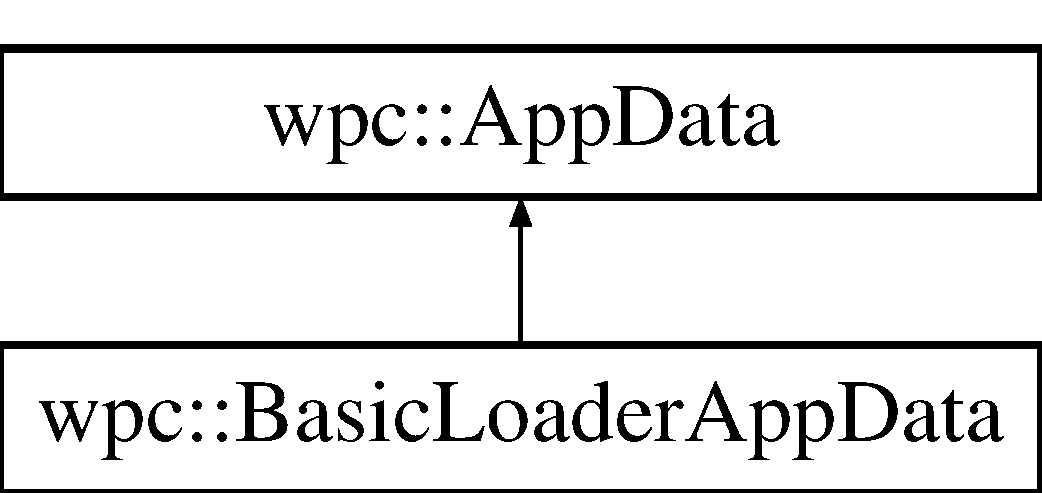
\includegraphics[height=2.000000cm]{structwpc_1_1_app_data}
\end{center}
\end{figure}
\subsection*{Public Member Functions}
\begin{DoxyCompactItemize}
\item 
virtual \hyperlink{structwpc_1_1_app_data_a053a227a398d2440bf7938a6fe33bdf0}{$\sim$\-App\-Data} ()
\end{DoxyCompactItemize}


\subsection{Detailed Description}
Interface for stucture describing application settings. 

Definition at line 41 of file loader\-\_\-traits.\-h.



\subsection{Constructor \& Destructor Documentation}
\hypertarget{structwpc_1_1_app_data_a053a227a398d2440bf7938a6fe33bdf0}{\index{wpc\-::\-App\-Data@{wpc\-::\-App\-Data}!$\sim$\-App\-Data@{$\sim$\-App\-Data}}
\index{$\sim$\-App\-Data@{$\sim$\-App\-Data}!wpc::AppData@{wpc\-::\-App\-Data}}
\subsubsection[{$\sim$\-App\-Data}]{\setlength{\rightskip}{0pt plus 5cm}virtual wpc\-::\-App\-Data\-::$\sim$\-App\-Data (
\begin{DoxyParamCaption}
{}
\end{DoxyParamCaption}
)\hspace{0.3cm}{\ttfamily [inline]}, {\ttfamily [virtual]}}}\label{structwpc_1_1_app_data_a053a227a398d2440bf7938a6fe33bdf0}


Definition at line 41 of file loader\-\_\-traits.\-h.



The documentation for this struct was generated from the following file\-:\begin{DoxyCompactItemize}
\item 
src/\hyperlink{loader__traits_8h}{loader\-\_\-traits.\-h}\end{DoxyCompactItemize}

\hypertarget{classwpc_1_1_basic_comparator}{\section{wpc\-:\-:Basic\-Comparator Class Reference}
\label{classwpc_1_1_basic_comparator}\index{wpc\-::\-Basic\-Comparator@{wpc\-::\-Basic\-Comparator}}
}


Defines basic class for comparison of two selected web page fragments.  




{\ttfamily \#include $<$Basic\-Comparator.\-h$>$}

\subsection*{Public Types}
\begin{DoxyCompactItemize}
\item 
enum \hyperlink{classwpc_1_1_basic_comparator_a95f6a6f66cb3a479371c101a35eebb6b}{C\-O\-L\-O\-R} \{ \hyperlink{classwpc_1_1_basic_comparator_a95f6a6f66cb3a479371c101a35eebb6ba8f07deb101c3ce46cdf92b7c4c14f01a}{R\-E\-D}, 
\hyperlink{classwpc_1_1_basic_comparator_a95f6a6f66cb3a479371c101a35eebb6bac4227992631e0fe13fcff5fafa0d2ea2}{G\-R\-E\-E\-N}, 
\hyperlink{classwpc_1_1_basic_comparator_a95f6a6f66cb3a479371c101a35eebb6baa4b78df226b5ed9886721fb9d81b7504}{B\-L\-U\-E}
 \}
\item 
typedef \hyperlink{structwpc_1_1cmp__trait}{cmp\-\_\-trait}\\*
$<$ \hyperlink{classwpc_1_1_basic_comparator}{Basic\-Comparator} $>$\\*
\-::\hyperlink{classwpc_1_1_basic_comparator_af93928e437d832b942be5396c4f453d1}{result\-\_\-type} \hyperlink{classwpc_1_1_basic_comparator_af93928e437d832b942be5396c4f453d1}{result\-\_\-type}
\begin{DoxyCompactList}\small\item\em Result type of operator() \mbox{[}required\mbox{]}. \end{DoxyCompactList}\end{DoxyCompactItemize}
\subsection*{Public Member Functions}
\begin{DoxyCompactItemize}
\item 
\hyperlink{classwpc_1_1_basic_comparator_af93928e437d832b942be5396c4f453d1}{result\-\_\-type} \hyperlink{classwpc_1_1_basic_comparator_aa73bc7915f828f313230c344fc2214cb}{operator()} (const cv\-::\-Mat \&larg, const cv\-::\-Mat \&parg)
\begin{DoxyCompactList}\small\item\em Operator() is being invoked by \hyperlink{classwpc_1_1_basic_loader}{Basic\-Loader} class to compare two images which are being considered as the same part of different web pages. \end{DoxyCompactList}\item 
\hyperlink{classwpc_1_1_basic_comparator_a319095093ff9a3411515721d73c1ba8d}{$\sim$\-Basic\-Comparator} ()
\end{DoxyCompactItemize}
\subsection*{Private Member Functions}
\begin{DoxyCompactItemize}
\item 
float \hyperlink{classwpc_1_1_basic_comparator_a2d12f50c780cf75e00c2e4aa0465a1f5}{calc\-Momentum} (const cv\-::\-Mat \&src, \hyperlink{classwpc_1_1_basic_comparator_a95f6a6f66cb3a479371c101a35eebb6b}{C\-O\-L\-O\-R} color, int axis=0)
\begin{DoxyCompactList}\small\item\em Calculates Co\-G of selected colour in respect for selected axis. \end{DoxyCompactList}\end{DoxyCompactItemize}


\subsection{Detailed Description}
Defines basic class for comparison of two selected web page fragments. 

Definition at line 53 of file Basic\-Comparator.\-h.



\subsection{Member Typedef Documentation}
\hypertarget{classwpc_1_1_basic_comparator_af93928e437d832b942be5396c4f453d1}{\index{wpc\-::\-Basic\-Comparator@{wpc\-::\-Basic\-Comparator}!result\-\_\-type@{result\-\_\-type}}
\index{result\-\_\-type@{result\-\_\-type}!wpc::BasicComparator@{wpc\-::\-Basic\-Comparator}}
\subsubsection[{result\-\_\-type}]{\setlength{\rightskip}{0pt plus 5cm}typedef {\bf cmp\-\_\-trait}$<${\bf Basic\-Comparator}$>$\-::{\bf result\-\_\-type} {\bf wpc\-::\-Basic\-Comparator\-::result\-\_\-type}}}\label{classwpc_1_1_basic_comparator_af93928e437d832b942be5396c4f453d1}


Result type of operator() \mbox{[}required\mbox{]}. 



Definition at line 61 of file Basic\-Comparator.\-h.



\subsection{Member Enumeration Documentation}
\hypertarget{classwpc_1_1_basic_comparator_a95f6a6f66cb3a479371c101a35eebb6b}{\index{wpc\-::\-Basic\-Comparator@{wpc\-::\-Basic\-Comparator}!C\-O\-L\-O\-R@{C\-O\-L\-O\-R}}
\index{C\-O\-L\-O\-R@{C\-O\-L\-O\-R}!wpc::BasicComparator@{wpc\-::\-Basic\-Comparator}}
\subsubsection[{C\-O\-L\-O\-R}]{\setlength{\rightskip}{0pt plus 5cm}enum {\bf wpc\-::\-Basic\-Comparator\-::\-C\-O\-L\-O\-R}}}\label{classwpc_1_1_basic_comparator_a95f6a6f66cb3a479371c101a35eebb6b}
\begin{Desc}
\item[Enumerator]\par
\begin{description}
\index{R\-E\-D@{R\-E\-D}!wpc\-::\-Basic\-Comparator@{wpc\-::\-Basic\-Comparator}}\index{wpc\-::\-Basic\-Comparator@{wpc\-::\-Basic\-Comparator}!R\-E\-D@{R\-E\-D}}\item[{\em 
\hypertarget{classwpc_1_1_basic_comparator_a95f6a6f66cb3a479371c101a35eebb6ba8f07deb101c3ce46cdf92b7c4c14f01a}{R\-E\-D}\label{classwpc_1_1_basic_comparator_a95f6a6f66cb3a479371c101a35eebb6ba8f07deb101c3ce46cdf92b7c4c14f01a}
}]\index{G\-R\-E\-E\-N@{G\-R\-E\-E\-N}!wpc\-::\-Basic\-Comparator@{wpc\-::\-Basic\-Comparator}}\index{wpc\-::\-Basic\-Comparator@{wpc\-::\-Basic\-Comparator}!G\-R\-E\-E\-N@{G\-R\-E\-E\-N}}\item[{\em 
\hypertarget{classwpc_1_1_basic_comparator_a95f6a6f66cb3a479371c101a35eebb6bac4227992631e0fe13fcff5fafa0d2ea2}{G\-R\-E\-E\-N}\label{classwpc_1_1_basic_comparator_a95f6a6f66cb3a479371c101a35eebb6bac4227992631e0fe13fcff5fafa0d2ea2}
}]Red channel \index{B\-L\-U\-E@{B\-L\-U\-E}!wpc\-::\-Basic\-Comparator@{wpc\-::\-Basic\-Comparator}}\index{wpc\-::\-Basic\-Comparator@{wpc\-::\-Basic\-Comparator}!B\-L\-U\-E@{B\-L\-U\-E}}\item[{\em 
\hypertarget{classwpc_1_1_basic_comparator_a95f6a6f66cb3a479371c101a35eebb6baa4b78df226b5ed9886721fb9d81b7504}{B\-L\-U\-E}\label{classwpc_1_1_basic_comparator_a95f6a6f66cb3a479371c101a35eebb6baa4b78df226b5ed9886721fb9d81b7504}
}]Green channel

Blue channel \end{description}
\end{Desc}


Definition at line 55 of file Basic\-Comparator.\-h.



\subsection{Constructor \& Destructor Documentation}
\hypertarget{classwpc_1_1_basic_comparator_a319095093ff9a3411515721d73c1ba8d}{\index{wpc\-::\-Basic\-Comparator@{wpc\-::\-Basic\-Comparator}!$\sim$\-Basic\-Comparator@{$\sim$\-Basic\-Comparator}}
\index{$\sim$\-Basic\-Comparator@{$\sim$\-Basic\-Comparator}!wpc::BasicComparator@{wpc\-::\-Basic\-Comparator}}
\subsubsection[{$\sim$\-Basic\-Comparator}]{\setlength{\rightskip}{0pt plus 5cm}wpc\-::\-Basic\-Comparator\-::$\sim$\-Basic\-Comparator (
\begin{DoxyParamCaption}
{}
\end{DoxyParamCaption}
)\hspace{0.3cm}{\ttfamily [inline]}}}\label{classwpc_1_1_basic_comparator_a319095093ff9a3411515721d73c1ba8d}
\begin{DoxyReturn}{Returns}
Comparison results 
\end{DoxyReturn}


Definition at line 68 of file Basic\-Comparator.\-h.



\subsection{Member Function Documentation}
\hypertarget{classwpc_1_1_basic_comparator_a2d12f50c780cf75e00c2e4aa0465a1f5}{\index{wpc\-::\-Basic\-Comparator@{wpc\-::\-Basic\-Comparator}!calc\-Momentum@{calc\-Momentum}}
\index{calc\-Momentum@{calc\-Momentum}!wpc::BasicComparator@{wpc\-::\-Basic\-Comparator}}
\subsubsection[{calc\-Momentum}]{\setlength{\rightskip}{0pt plus 5cm}float wpc\-::\-Basic\-Comparator\-::calc\-Momentum (
\begin{DoxyParamCaption}
\item[{const cv\-::\-Mat \&}]{src, }
\item[{{\bf C\-O\-L\-O\-R}}]{color, }
\item[{int}]{axis = {\ttfamily 0}}
\end{DoxyParamCaption}
)\hspace{0.3cm}{\ttfamily [private]}}}\label{classwpc_1_1_basic_comparator_a2d12f50c780cf75e00c2e4aa0465a1f5}


Calculates Co\-G of selected colour in respect for selected axis. 

Calculates specified color Co\-G with respect to appropriate axis.


\begin{DoxyParams}[1]{Parameters}
\mbox{\tt in}  & {\em src} & -\/ source matrix \\
\hline
\mbox{\tt in}  & {\em color} & -\/ selected channel see \hyperlink{classwpc_1_1_basic_comparator_a95f6a6f66cb3a479371c101a35eebb6b}{C\-O\-L\-O\-R} \\
\hline
\mbox{\tt in}  & {\em axis} & -\/ selected image axis (X or Y) By default 0 means X.\\
\hline
\mbox{\tt in}  & {\em src} & -\/ source matrix (3 channels) \\
\hline
\mbox{\tt in}  & {\em color} & -\/ color (see \hyperlink{classwpc_1_1_basic_comparator_a95f6a6f66cb3a479371c101a35eebb6b}{Basic\-Comparator\-::\-C\-O\-L\-O\-R} ) \\
\hline
\mbox{\tt in}  & {\em axis} & -\/ specified axis \\
\hline
\end{DoxyParams}


Definition at line 44 of file Basic\-Comparator.\-cpp.

\hypertarget{classwpc_1_1_basic_comparator_aa73bc7915f828f313230c344fc2214cb}{\index{wpc\-::\-Basic\-Comparator@{wpc\-::\-Basic\-Comparator}!operator()@{operator()}}
\index{operator()@{operator()}!wpc::BasicComparator@{wpc\-::\-Basic\-Comparator}}
\subsubsection[{operator()}]{\setlength{\rightskip}{0pt plus 5cm}{\bf Basic\-Comparator\-::result\-\_\-type} wpc\-::\-Basic\-Comparator\-::operator() (
\begin{DoxyParamCaption}
\item[{const cv\-::\-Mat \&}]{larg, }
\item[{const cv\-::\-Mat \&}]{parg}
\end{DoxyParamCaption}
)}}\label{classwpc_1_1_basic_comparator_aa73bc7915f828f313230c344fc2214cb}


Operator() is being invoked by \hyperlink{classwpc_1_1_basic_loader}{Basic\-Loader} class to compare two images which are being considered as the same part of different web pages. 

Compares given images calculating maximum distance between centers of colours in 3\-D space.


\begin{DoxyParams}[1]{Parameters}
\mbox{\tt in}  & {\em larg} & -\/ first image \\
\hline
\mbox{\tt in}  & {\em parg} & -\/ second image \\
\hline
\end{DoxyParams}
\begin{DoxyReturn}{Returns}
distance between centers of colours in 3\-D space. 
\end{DoxyReturn}


Definition at line 89 of file Basic\-Comparator.\-cpp.



The documentation for this class was generated from the following files\-:\begin{DoxyCompactItemize}
\item 
src/\hyperlink{_basic_comparator_8h}{Basic\-Comparator.\-h}\item 
src/\hyperlink{_basic_comparator_8cpp}{Basic\-Comparator.\-cpp}\end{DoxyCompactItemize}

\hypertarget{classwpc_1_1_basic_loader}{\section{wpc\-:\-:Basic\-Loader Class Reference}
\label{classwpc_1_1_basic_loader}\index{wpc\-::\-Basic\-Loader@{wpc\-::\-Basic\-Loader}}
}


Loads and carryies out the comparison process.  




{\ttfamily \#include $<$Basic\-Loader.\-h$>$}

\subsection*{Public Types}
\begin{DoxyCompactItemize}
\item 
typedef std\-::vector$<$ \hyperlink{structwpc_1_1_result_type}{Result\-Type} $>$ \hyperlink{classwpc_1_1_basic_loader_abae37c020f8996c8cd770db2edcb3bea}{Comparison\-Result\-Type}
\end{DoxyCompactItemize}
\subsection*{Public Member Functions}
\begin{DoxyCompactItemize}
\item 
\hyperlink{classwpc_1_1_basic_loader_aad2a76648585da05f702e8b456ed9771}{Basic\-Loader} ()
\item 
void \hyperlink{classwpc_1_1_basic_loader_a05153c89ee24cb38447a04215c58e488}{operator()} (\hyperlink{structwpc_1_1_app_data}{App\-Data} \&app\-Data)
\begin{DoxyCompactList}\small\item\em Operator() is responsible for loading specified browsers and starting comparison process using provided \hyperlink{classwpc_1_1_basic_comparator}{Basic\-Comparator} object. \end{DoxyCompactList}\item 
void \hyperlink{classwpc_1_1_basic_loader_ad99e8b8031a9757179361e24676c4fdc}{set\-Comparator\-Object} (const \hyperlink{structwpc_1_1cmp__trait}{cmp\-\_\-trait}$<$ \hyperlink{classwpc_1_1_basic_comparator}{Basic\-Comparator} $>$\-::cmp\-\_\-call\-\_\-sig \&st)
\begin{DoxyCompactList}\small\item\em Sets comparator object. \end{DoxyCompactList}\item 
const \hyperlink{classwpc_1_1_basic_loader_abae37c020f8996c8cd770db2edcb3bea}{Comparison\-Result\-Type} \& \hyperlink{classwpc_1_1_basic_loader_a95212e768136af62abb7db739dd7cc9b}{get\-Results} () const 
\item 
\hyperlink{classwpc_1_1_basic_loader_a0da11cf2fb72e7706fd878b71dd303f5}{$\sim$\-Basic\-Loader} ()
\end{DoxyCompactItemize}
\subsection*{Private Member Functions}
\begin{DoxyCompactItemize}
\item 
void \hyperlink{classwpc_1_1_basic_loader_a5d58596278a4f9ffc1100bae2a37b4a5}{to\-Mat} (int, cv\-::\-Mat \&Screen) const 
\begin{DoxyCompactList}\small\item\em \mbox{[}Linux\mbox{]} Not supported yet. \end{DoxyCompactList}\item 
void \hyperlink{classwpc_1_1_basic_loader_a715fa2e450294b3c8ada601d720bd236}{run} (\hyperlink{structwpc_1_1_app_data}{App\-Data} \&)
\begin{DoxyCompactList}\small\item\em Same as operator() \end{DoxyCompactList}\item 
bool \hyperlink{classwpc_1_1_basic_loader_a760546ee7fb17cf593401a15beb5a30e}{start} (\hyperlink{structwpc_1_1_browser_data}{Browser\-Data} \&application, const std\-::string \&file\-Name)
\begin{DoxyCompactList}\small\item\em Starts browsers. Function launches specified web browser with additional parameter \char`\"{}filename\char`\"{}. \end{DoxyCompactList}\item 
void \hyperlink{classwpc_1_1_basic_loader_ac562a2638ad95b3711f2ea63ba7719e4}{close\-Browsers} (const \hyperlink{structwpc_1_1_browser_data}{Browser\-Data} \&bd) const 
\begin{DoxyCompactList}\small\item\em Closes started browsers afer comparison. \end{DoxyCompactList}\item 
void \hyperlink{classwpc_1_1_basic_loader_a1197416ed7fda5cebe773ed9bc12d323}{compare\-Pages} (const \hyperlink{structwpc_1_1_basic_loader_app_data}{Basic\-Loader\-App\-Data} \&pg)
\begin{DoxyCompactList}\small\item\em Compares pages using selected comparator. \end{DoxyCompactList}\item 
void \hyperlink{classwpc_1_1_basic_loader_a4bd3ad5553e97dd14dcffec70d4696a7}{acquire\-Layers} (int i, const \hyperlink{structwpc_1_1_basic_loader_app_data}{Basic\-Loader\-App\-Data} \&pg, \hyperlink{namespacewpc_a778a3f9b2be5b4dd228ea2c752dc7aa2}{Layer\-Data\-Vector} \&layers)
\begin{DoxyCompactList}\small\item\em Acquires specified layer from web browser as a screen shot. \end{DoxyCompactList}\item 
bool \hyperlink{classwpc_1_1_basic_loader_a0ab4391f59be82bab93b8e248f689a96}{loc\-R\-O\-I} (const cv\-::\-Mat \&mask, cv\-::\-Point \&P1, cv\-::\-Point \&P2)
\begin{DoxyCompactList}\small\item\em Localizes R\-O\-I in provided image. R\-O\-I is being described using specified colour. \end{DoxyCompactList}\item 
cv\-::\-Mat $\ast$ \hyperlink{classwpc_1_1_basic_loader_ac16dabc4773e364f56aabe52c7d8d93e}{get\-Image} (const \hyperlink{structwpc_1_1_layer_data}{Layer\-Data} \&object, const \hyperlink{namespacewpc_a778a3f9b2be5b4dd228ea2c752dc7aa2}{Layer\-Data\-Vector} \&array) const 
\begin{DoxyCompactList}\small\item\em Retrieves associated image from an array using browser description. \end{DoxyCompactList}\end{DoxyCompactItemize}
\subsection*{Private Attributes}
\begin{DoxyCompactItemize}
\item 
int \hyperlink{classwpc_1_1_basic_loader_a3b78c6d764a8ee7985b7ec471eb9d276}{m\-\_\-layer\-Number}
\item 
int \hyperlink{classwpc_1_1_basic_loader_afc1f23543a23f8f3afbec0b9d6d8837e}{m\-\_\-counter\-Initial}
\item 
int \hyperlink{classwpc_1_1_basic_loader_a9d5e11507f6111f601016f1b06b2eecd}{m\-\_\-layer\-Change\-Delay}
\item 
\hyperlink{classwpc_1_1_basic_options}{Basic\-Options} \hyperlink{classwpc_1_1_basic_loader_a869f709a80ee7a0c5a47d12c11fc4d14}{m\-\_\-options}
\item 
\hyperlink{classwpc_1_1_basic_loader_abae37c020f8996c8cd770db2edcb3bea}{Comparison\-Result\-Type} \hyperlink{classwpc_1_1_basic_loader_a7b03bfcc76578e8a45b1f70495541b72}{m\-\_\-results}
\item 
\hyperlink{structwpc_1_1cmp__trait}{cmp\-\_\-trait}$<$ \hyperlink{classwpc_1_1_basic_comparator}{Basic\-Comparator} $>$\\*
\-::cmp\-\_\-call\-\_\-sig \hyperlink{classwpc_1_1_basic_loader_a6ce950ebdb25b76dafde911ca69bfced}{comparator}
\end{DoxyCompactItemize}
\subsection*{Static Private Attributes}
\begin{DoxyCompactItemize}
\item 
static std\-::string \hyperlink{classwpc_1_1_basic_loader_a2fb7543b8e4b8b11c55727cc12115f83}{m\-\_\-js\-Script\-Name} = \char`\"{}data/default/hscript.\-js\char`\"{}
\begin{DoxyCompactList}\small\item\em Describes name of Java\-Script file, responsible for highlightning layers. \end{DoxyCompactList}\item 
static std\-::string \hyperlink{classwpc_1_1_basic_loader_ae160d8e7f8dd2e463ee6ccddc7c34073}{m\-\_\-\-Temp\-Name} = \char`\"{}temporary.\-html\char`\"{}
\begin{DoxyCompactList}\small\item\em Temporary name of. \end{DoxyCompactList}\end{DoxyCompactItemize}


\subsection{Detailed Description}
Loads and carryies out the comparison process. 

Class is being used for loading (starting browsers) and carrying out the process of cross browser validation using specified methods (in default solution provided by Basic\-Comparison class). 

Definition at line 100 of file Basic\-Loader.\-h.



\subsection{Member Typedef Documentation}
\hypertarget{classwpc_1_1_basic_loader_abae37c020f8996c8cd770db2edcb3bea}{\index{wpc\-::\-Basic\-Loader@{wpc\-::\-Basic\-Loader}!Comparison\-Result\-Type@{Comparison\-Result\-Type}}
\index{Comparison\-Result\-Type@{Comparison\-Result\-Type}!wpc::BasicLoader@{wpc\-::\-Basic\-Loader}}
\subsubsection[{Comparison\-Result\-Type}]{\setlength{\rightskip}{0pt plus 5cm}typedef std\-::vector$<${\bf Result\-Type}$>$ {\bf wpc\-::\-Basic\-Loader\-::\-Comparison\-Result\-Type}}}\label{classwpc_1_1_basic_loader_abae37c020f8996c8cd770db2edcb3bea}


Definition at line 102 of file Basic\-Loader.\-h.



\subsection{Constructor \& Destructor Documentation}
\hypertarget{classwpc_1_1_basic_loader_aad2a76648585da05f702e8b456ed9771}{\index{wpc\-::\-Basic\-Loader@{wpc\-::\-Basic\-Loader}!Basic\-Loader@{Basic\-Loader}}
\index{Basic\-Loader@{Basic\-Loader}!wpc::BasicLoader@{wpc\-::\-Basic\-Loader}}
\subsubsection[{Basic\-Loader}]{\setlength{\rightskip}{0pt plus 5cm}wpc\-::\-Basic\-Loader\-::\-Basic\-Loader (
\begin{DoxyParamCaption}
{}
\end{DoxyParamCaption}
)\hspace{0.3cm}{\ttfamily [inline]}}}\label{classwpc_1_1_basic_loader_aad2a76648585da05f702e8b456ed9771}


Definition at line 103 of file Basic\-Loader.\-h.

\hypertarget{classwpc_1_1_basic_loader_a0da11cf2fb72e7706fd878b71dd303f5}{\index{wpc\-::\-Basic\-Loader@{wpc\-::\-Basic\-Loader}!$\sim$\-Basic\-Loader@{$\sim$\-Basic\-Loader}}
\index{$\sim$\-Basic\-Loader@{$\sim$\-Basic\-Loader}!wpc::BasicLoader@{wpc\-::\-Basic\-Loader}}
\subsubsection[{$\sim$\-Basic\-Loader}]{\setlength{\rightskip}{0pt plus 5cm}wpc\-::\-Basic\-Loader\-::$\sim$\-Basic\-Loader (
\begin{DoxyParamCaption}
{}
\end{DoxyParamCaption}
)\hspace{0.3cm}{\ttfamily [inline]}}}\label{classwpc_1_1_basic_loader_a0da11cf2fb72e7706fd878b71dd303f5}


Definition at line 122 of file Basic\-Loader.\-h.



\subsection{Member Function Documentation}
\hypertarget{classwpc_1_1_basic_loader_a4bd3ad5553e97dd14dcffec70d4696a7}{\index{wpc\-::\-Basic\-Loader@{wpc\-::\-Basic\-Loader}!acquire\-Layers@{acquire\-Layers}}
\index{acquire\-Layers@{acquire\-Layers}!wpc::BasicLoader@{wpc\-::\-Basic\-Loader}}
\subsubsection[{acquire\-Layers}]{\setlength{\rightskip}{0pt plus 5cm}void wpc\-::\-Basic\-Loader\-::acquire\-Layers (
\begin{DoxyParamCaption}
\item[{int}]{i, }
\item[{const {\bf Basic\-Loader\-App\-Data} \&}]{pg, }
\item[{{\bf Layer\-Data\-Vector} \&}]{layers}
\end{DoxyParamCaption}
)\hspace{0.3cm}{\ttfamily [private]}}}\label{classwpc_1_1_basic_loader_a4bd3ad5553e97dd14dcffec70d4696a7}


Acquires specified layer from web browser as a screen shot. 


\begin{DoxyParams}[1]{Parameters}
\mbox{\tt in}  & {\em i} & -\/ layer number \\
\hline
\mbox{\tt in}  & {\em pg} & -\/ list of browsers to compare \\
\hline
\mbox{\tt in}  & {\em layers} & -\/ descriptor (image,browser) \\
\hline
\end{DoxyParams}


Definition at line 163 of file Basic\-Loader.\-cpp.

\hypertarget{classwpc_1_1_basic_loader_ac562a2638ad95b3711f2ea63ba7719e4}{\index{wpc\-::\-Basic\-Loader@{wpc\-::\-Basic\-Loader}!close\-Browsers@{close\-Browsers}}
\index{close\-Browsers@{close\-Browsers}!wpc::BasicLoader@{wpc\-::\-Basic\-Loader}}
\subsubsection[{close\-Browsers}]{\setlength{\rightskip}{0pt plus 5cm}void wpc\-::\-Basic\-Loader\-::close\-Browsers (
\begin{DoxyParamCaption}
\item[{const {\bf Browser\-Data} \&}]{bd}
\end{DoxyParamCaption}
) const\hspace{0.3cm}{\ttfamily [private]}}}\label{classwpc_1_1_basic_loader_ac562a2638ad95b3711f2ea63ba7719e4}


Closes started browsers afer comparison. 


\begin{DoxyParams}[1]{Parameters}
\mbox{\tt in}  & {\em bd} & -\/ descriptor of a single web browser \\
\hline
\end{DoxyParams}


Definition at line 110 of file Basic\-Loader.\-cpp.

\hypertarget{classwpc_1_1_basic_loader_a1197416ed7fda5cebe773ed9bc12d323}{\index{wpc\-::\-Basic\-Loader@{wpc\-::\-Basic\-Loader}!compare\-Pages@{compare\-Pages}}
\index{compare\-Pages@{compare\-Pages}!wpc::BasicLoader@{wpc\-::\-Basic\-Loader}}
\subsubsection[{compare\-Pages}]{\setlength{\rightskip}{0pt plus 5cm}void wpc\-::\-Basic\-Loader\-::compare\-Pages (
\begin{DoxyParamCaption}
\item[{const {\bf Basic\-Loader\-App\-Data} \&}]{pg}
\end{DoxyParamCaption}
)\hspace{0.3cm}{\ttfamily [private]}}}\label{classwpc_1_1_basic_loader_a1197416ed7fda5cebe773ed9bc12d323}


Compares pages using selected comparator. 


\begin{DoxyParams}[1]{Parameters}
\mbox{\tt in}  & {\em pg} & -\/ defines list of browsers which should be compared \\
\hline
\end{DoxyParams}


Definition at line 125 of file Basic\-Loader.\-cpp.

\hypertarget{classwpc_1_1_basic_loader_ac16dabc4773e364f56aabe52c7d8d93e}{\index{wpc\-::\-Basic\-Loader@{wpc\-::\-Basic\-Loader}!get\-Image@{get\-Image}}
\index{get\-Image@{get\-Image}!wpc::BasicLoader@{wpc\-::\-Basic\-Loader}}
\subsubsection[{get\-Image}]{\setlength{\rightskip}{0pt plus 5cm}cv\-::\-Mat $\ast$ wpc\-::\-Basic\-Loader\-::get\-Image (
\begin{DoxyParamCaption}
\item[{const {\bf Layer\-Data} \&}]{object, }
\item[{const {\bf Layer\-Data\-Vector} \&}]{array}
\end{DoxyParamCaption}
) const\hspace{0.3cm}{\ttfamily [private]}}}\label{classwpc_1_1_basic_loader_ac16dabc4773e364f56aabe52c7d8d93e}


Retrieves associated image from an array using browser description. 


\begin{DoxyParams}[1]{Parameters}
\mbox{\tt in}  & {\em object} & -\/ describes particular browser \\
\hline
\mbox{\tt in}  & {\em array} & -\/ array of objects \\
\hline
\end{DoxyParams}


Definition at line 117 of file Basic\-Loader.\-cpp.

\hypertarget{classwpc_1_1_basic_loader_a95212e768136af62abb7db739dd7cc9b}{\index{wpc\-::\-Basic\-Loader@{wpc\-::\-Basic\-Loader}!get\-Results@{get\-Results}}
\index{get\-Results@{get\-Results}!wpc::BasicLoader@{wpc\-::\-Basic\-Loader}}
\subsubsection[{get\-Results}]{\setlength{\rightskip}{0pt plus 5cm}const {\bf Basic\-Loader\-::\-Comparison\-Result\-Type} \& wpc\-::\-Basic\-Loader\-::get\-Results (
\begin{DoxyParamCaption}
{}
\end{DoxyParamCaption}
) const\hspace{0.3cm}{\ttfamily [inline]}}}\label{classwpc_1_1_basic_loader_a95212e768136af62abb7db739dd7cc9b}


Definition at line 202 of file Basic\-Loader.\-h.

\hypertarget{classwpc_1_1_basic_loader_a0ab4391f59be82bab93b8e248f689a96}{\index{wpc\-::\-Basic\-Loader@{wpc\-::\-Basic\-Loader}!loc\-R\-O\-I@{loc\-R\-O\-I}}
\index{loc\-R\-O\-I@{loc\-R\-O\-I}!wpc::BasicLoader@{wpc\-::\-Basic\-Loader}}
\subsubsection[{loc\-R\-O\-I}]{\setlength{\rightskip}{0pt plus 5cm}bool wpc\-::\-Basic\-Loader\-::loc\-R\-O\-I (
\begin{DoxyParamCaption}
\item[{const cv\-::\-Mat \&}]{mask, }
\item[{cv\-::\-Point \&}]{P1, }
\item[{cv\-::\-Point \&}]{P2}
\end{DoxyParamCaption}
)\hspace{0.3cm}{\ttfamily [private]}}}\label{classwpc_1_1_basic_loader_a0ab4391f59be82bab93b8e248f689a96}


Localizes R\-O\-I in provided image. R\-O\-I is being described using specified colour. 


\begin{DoxyParams}[1]{Parameters}
\mbox{\tt in}  & {\em mask} & -\/ image with highlighted R\-O\-I \\
\hline
\mbox{\tt out}  & {\em P1} & -\/ coordinates of left upper corner of found R\-O\-I \\
\hline
\mbox{\tt out}  & {\em P2} & -\/ coordinates of left upper corner of found R\-O\-I \\
\hline
\end{DoxyParams}


Definition at line 47 of file Basic\-Loader.\-cpp.

\hypertarget{classwpc_1_1_basic_loader_a05153c89ee24cb38447a04215c58e488}{\index{wpc\-::\-Basic\-Loader@{wpc\-::\-Basic\-Loader}!operator()@{operator()}}
\index{operator()@{operator()}!wpc::BasicLoader@{wpc\-::\-Basic\-Loader}}
\subsubsection[{operator()}]{\setlength{\rightskip}{0pt plus 5cm}void wpc\-::\-Basic\-Loader\-::operator() (
\begin{DoxyParamCaption}
\item[{{\bf App\-Data} \&}]{app\-Data}
\end{DoxyParamCaption}
)}}\label{classwpc_1_1_basic_loader_a05153c89ee24cb38447a04215c58e488}


Operator() is responsible for loading specified browsers and starting comparison process using provided \hyperlink{classwpc_1_1_basic_comparator}{Basic\-Comparator} object. 


\begin{DoxyParams}[1]{Parameters}
\mbox{\tt in}  & {\em app\-Data} & -\/ list specifing paths/titles of the browsers to be started. For further details see \hyperlink{structwpc_1_1_basic_loader_app_data}{Basic\-Loader\-App\-Data} \\
\hline
\end{DoxyParams}


Definition at line 263 of file Basic\-Loader.\-cpp.

\hypertarget{classwpc_1_1_basic_loader_a715fa2e450294b3c8ada601d720bd236}{\index{wpc\-::\-Basic\-Loader@{wpc\-::\-Basic\-Loader}!run@{run}}
\index{run@{run}!wpc::BasicLoader@{wpc\-::\-Basic\-Loader}}
\subsubsection[{run}]{\setlength{\rightskip}{0pt plus 5cm}void wpc\-::\-Basic\-Loader\-::run (
\begin{DoxyParamCaption}
\item[{{\bf App\-Data} \&}]{app\-Paths}
\end{DoxyParamCaption}
)\hspace{0.3cm}{\ttfamily [private]}}}\label{classwpc_1_1_basic_loader_a715fa2e450294b3c8ada601d720bd236}


Same as operator() 



Definition at line 211 of file Basic\-Loader.\-cpp.

\hypertarget{classwpc_1_1_basic_loader_ad99e8b8031a9757179361e24676c4fdc}{\index{wpc\-::\-Basic\-Loader@{wpc\-::\-Basic\-Loader}!set\-Comparator\-Object@{set\-Comparator\-Object}}
\index{set\-Comparator\-Object@{set\-Comparator\-Object}!wpc::BasicLoader@{wpc\-::\-Basic\-Loader}}
\subsubsection[{set\-Comparator\-Object}]{\setlength{\rightskip}{0pt plus 5cm}void wpc\-::\-Basic\-Loader\-::set\-Comparator\-Object (
\begin{DoxyParamCaption}
\item[{const {\bf cmp\-\_\-trait}$<$ {\bf Basic\-Comparator} $>$\-::cmp\-\_\-call\-\_\-sig \&}]{st}
\end{DoxyParamCaption}
)\hspace{0.3cm}{\ttfamily [inline]}}}\label{classwpc_1_1_basic_loader_ad99e8b8031a9757179361e24676c4fdc}


Sets comparator object. 

Sets the comparison object used for comparing selected parts of web page.


\begin{DoxyParams}[1]{Parameters}
 & {\em st} & -\/ slot based on boost\-::signals2 library providing call to operator() of \hyperlink{classwpc_1_1_basic_comparator}{Basic\-Comparator}\\
\hline
\mbox{\tt in}  & {\em st} & -\/ comparison object \\
\hline
\end{DoxyParams}


Definition at line 211 of file Basic\-Loader.\-h.

\hypertarget{classwpc_1_1_basic_loader_a760546ee7fb17cf593401a15beb5a30e}{\index{wpc\-::\-Basic\-Loader@{wpc\-::\-Basic\-Loader}!start@{start}}
\index{start@{start}!wpc::BasicLoader@{wpc\-::\-Basic\-Loader}}
\subsubsection[{start}]{\setlength{\rightskip}{0pt plus 5cm}bool wpc\-::\-Basic\-Loader\-::start (
\begin{DoxyParamCaption}
\item[{{\bf Browser\-Data} \&}]{application, }
\item[{const std\-::string \&}]{file\-Name}
\end{DoxyParamCaption}
)\hspace{0.3cm}{\ttfamily [private]}}}\label{classwpc_1_1_basic_loader_a760546ee7fb17cf593401a15beb5a30e}


Starts browsers. Function launches specified web browser with additional parameter \char`\"{}filename\char`\"{}. 


\begin{DoxyParams}[1]{Parameters}
\mbox{\tt in}  & {\em application} & -\/ browser descriptor see\-: \hyperlink{structwpc_1_1_browser_data}{Browser\-Data} \\
\hline
\mbox{\tt in}  & {\em file\-Name} & -\/ name of file to start \\
\hline
\end{DoxyParams}


Definition at line 189 of file Basic\-Loader.\-cpp.

\hypertarget{classwpc_1_1_basic_loader_a5d58596278a4f9ffc1100bae2a37b4a5}{\index{wpc\-::\-Basic\-Loader@{wpc\-::\-Basic\-Loader}!to\-Mat@{to\-Mat}}
\index{to\-Mat@{to\-Mat}!wpc::BasicLoader@{wpc\-::\-Basic\-Loader}}
\subsubsection[{to\-Mat}]{\setlength{\rightskip}{0pt plus 5cm}void wpc\-::\-Basic\-Loader\-::to\-Mat (
\begin{DoxyParamCaption}
\item[{int}]{, }
\item[{cv\-::\-Mat \&}]{Screen}
\end{DoxyParamCaption}
) const\hspace{0.3cm}{\ttfamily [private]}}}\label{classwpc_1_1_basic_loader_a5d58596278a4f9ffc1100bae2a37b4a5}


\mbox{[}Linux\mbox{]} Not supported yet. 



Definition at line 105 of file Basic\-Loader.\-cpp.



\subsection{Member Data Documentation}
\hypertarget{classwpc_1_1_basic_loader_a6ce950ebdb25b76dafde911ca69bfced}{\index{wpc\-::\-Basic\-Loader@{wpc\-::\-Basic\-Loader}!comparator@{comparator}}
\index{comparator@{comparator}!wpc::BasicLoader@{wpc\-::\-Basic\-Loader}}
\subsubsection[{comparator}]{\setlength{\rightskip}{0pt plus 5cm}{\bf cmp\-\_\-trait}$<${\bf Basic\-Comparator}$>$\-::cmp\-\_\-call\-\_\-sig wpc\-::\-Basic\-Loader\-::comparator\hspace{0.3cm}{\ttfamily [private]}}}\label{classwpc_1_1_basic_loader_a6ce950ebdb25b76dafde911ca69bfced}


Definition at line 199 of file Basic\-Loader.\-h.

\hypertarget{classwpc_1_1_basic_loader_afc1f23543a23f8f3afbec0b9d6d8837e}{\index{wpc\-::\-Basic\-Loader@{wpc\-::\-Basic\-Loader}!m\-\_\-counter\-Initial@{m\-\_\-counter\-Initial}}
\index{m\-\_\-counter\-Initial@{m\-\_\-counter\-Initial}!wpc::BasicLoader@{wpc\-::\-Basic\-Loader}}
\subsubsection[{m\-\_\-counter\-Initial}]{\setlength{\rightskip}{0pt plus 5cm}int wpc\-::\-Basic\-Loader\-::m\-\_\-counter\-Initial\hspace{0.3cm}{\ttfamily [private]}}}\label{classwpc_1_1_basic_loader_afc1f23543a23f8f3afbec0b9d6d8837e}


Definition at line 125 of file Basic\-Loader.\-h.

\hypertarget{classwpc_1_1_basic_loader_a2fb7543b8e4b8b11c55727cc12115f83}{\index{wpc\-::\-Basic\-Loader@{wpc\-::\-Basic\-Loader}!m\-\_\-js\-Script\-Name@{m\-\_\-js\-Script\-Name}}
\index{m\-\_\-js\-Script\-Name@{m\-\_\-js\-Script\-Name}!wpc::BasicLoader@{wpc\-::\-Basic\-Loader}}
\subsubsection[{m\-\_\-js\-Script\-Name}]{\setlength{\rightskip}{0pt plus 5cm}std\-::string wpc\-::\-Basic\-Loader\-::m\-\_\-js\-Script\-Name = \char`\"{}data/default/hscript.\-js\char`\"{}\hspace{0.3cm}{\ttfamily [static]}, {\ttfamily [private]}}}\label{classwpc_1_1_basic_loader_a2fb7543b8e4b8b11c55727cc12115f83}


Describes name of Java\-Script file, responsible for highlightning layers. 



Definition at line 130 of file Basic\-Loader.\-h.

\hypertarget{classwpc_1_1_basic_loader_a9d5e11507f6111f601016f1b06b2eecd}{\index{wpc\-::\-Basic\-Loader@{wpc\-::\-Basic\-Loader}!m\-\_\-layer\-Change\-Delay@{m\-\_\-layer\-Change\-Delay}}
\index{m\-\_\-layer\-Change\-Delay@{m\-\_\-layer\-Change\-Delay}!wpc::BasicLoader@{wpc\-::\-Basic\-Loader}}
\subsubsection[{m\-\_\-layer\-Change\-Delay}]{\setlength{\rightskip}{0pt plus 5cm}int wpc\-::\-Basic\-Loader\-::m\-\_\-layer\-Change\-Delay\hspace{0.3cm}{\ttfamily [private]}}}\label{classwpc_1_1_basic_loader_a9d5e11507f6111f601016f1b06b2eecd}


Definition at line 126 of file Basic\-Loader.\-h.

\hypertarget{classwpc_1_1_basic_loader_a3b78c6d764a8ee7985b7ec471eb9d276}{\index{wpc\-::\-Basic\-Loader@{wpc\-::\-Basic\-Loader}!m\-\_\-layer\-Number@{m\-\_\-layer\-Number}}
\index{m\-\_\-layer\-Number@{m\-\_\-layer\-Number}!wpc::BasicLoader@{wpc\-::\-Basic\-Loader}}
\subsubsection[{m\-\_\-layer\-Number}]{\setlength{\rightskip}{0pt plus 5cm}int wpc\-::\-Basic\-Loader\-::m\-\_\-layer\-Number\hspace{0.3cm}{\ttfamily [private]}}}\label{classwpc_1_1_basic_loader_a3b78c6d764a8ee7985b7ec471eb9d276}


Definition at line 124 of file Basic\-Loader.\-h.

\hypertarget{classwpc_1_1_basic_loader_a869f709a80ee7a0c5a47d12c11fc4d14}{\index{wpc\-::\-Basic\-Loader@{wpc\-::\-Basic\-Loader}!m\-\_\-options@{m\-\_\-options}}
\index{m\-\_\-options@{m\-\_\-options}!wpc::BasicLoader@{wpc\-::\-Basic\-Loader}}
\subsubsection[{m\-\_\-options}]{\setlength{\rightskip}{0pt plus 5cm}{\bf Basic\-Options} wpc\-::\-Basic\-Loader\-::m\-\_\-options\hspace{0.3cm}{\ttfamily [private]}}}\label{classwpc_1_1_basic_loader_a869f709a80ee7a0c5a47d12c11fc4d14}


Definition at line 127 of file Basic\-Loader.\-h.

\hypertarget{classwpc_1_1_basic_loader_a7b03bfcc76578e8a45b1f70495541b72}{\index{wpc\-::\-Basic\-Loader@{wpc\-::\-Basic\-Loader}!m\-\_\-results@{m\-\_\-results}}
\index{m\-\_\-results@{m\-\_\-results}!wpc::BasicLoader@{wpc\-::\-Basic\-Loader}}
\subsubsection[{m\-\_\-results}]{\setlength{\rightskip}{0pt plus 5cm}{\bf Comparison\-Result\-Type} wpc\-::\-Basic\-Loader\-::m\-\_\-results\hspace{0.3cm}{\ttfamily [private]}}}\label{classwpc_1_1_basic_loader_a7b03bfcc76578e8a45b1f70495541b72}


Definition at line 128 of file Basic\-Loader.\-h.

\hypertarget{classwpc_1_1_basic_loader_ae160d8e7f8dd2e463ee6ccddc7c34073}{\index{wpc\-::\-Basic\-Loader@{wpc\-::\-Basic\-Loader}!m\-\_\-\-Temp\-Name@{m\-\_\-\-Temp\-Name}}
\index{m\-\_\-\-Temp\-Name@{m\-\_\-\-Temp\-Name}!wpc::BasicLoader@{wpc\-::\-Basic\-Loader}}
\subsubsection[{m\-\_\-\-Temp\-Name}]{\setlength{\rightskip}{0pt plus 5cm}std\-::string wpc\-::\-Basic\-Loader\-::m\-\_\-\-Temp\-Name = \char`\"{}temporary.\-html\char`\"{}\hspace{0.3cm}{\ttfamily [static]}, {\ttfamily [private]}}}\label{classwpc_1_1_basic_loader_ae160d8e7f8dd2e463ee6ccddc7c34073}


Temporary name of. 



Definition at line 132 of file Basic\-Loader.\-h.



The documentation for this class was generated from the following files\-:\begin{DoxyCompactItemize}
\item 
src/\hyperlink{_basic_loader_8h}{Basic\-Loader.\-h}\item 
src/\hyperlink{_basic_loader_8cpp}{Basic\-Loader.\-cpp}\end{DoxyCompactItemize}

\hypertarget{structwpc_1_1_basic_loader_app_data}{\section{wpc\-:\-:Basic\-Loader\-App\-Data Struct Reference}
\label{structwpc_1_1_basic_loader_app_data}\index{wpc\-::\-Basic\-Loader\-App\-Data@{wpc\-::\-Basic\-Loader\-App\-Data}}
}


Multiple browser descriptor for \hyperlink{classwpc_1_1_basic_loader}{Basic\-Loader}.  




{\ttfamily \#include $<$Basic\-Loader.\-h$>$}

Inheritance diagram for wpc\-:\-:Basic\-Loader\-App\-Data\-:\begin{figure}[H]
\begin{center}
\leavevmode
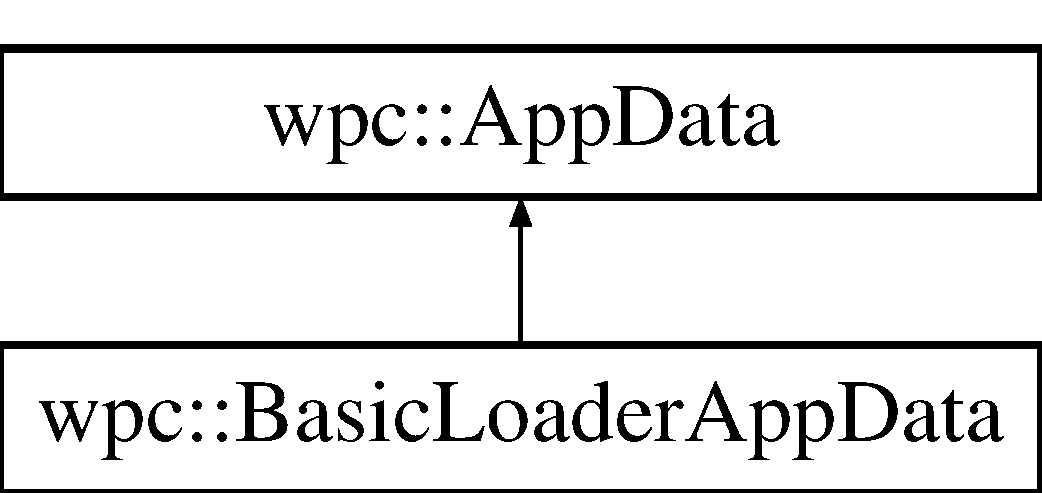
\includegraphics[height=2.000000cm]{structwpc_1_1_basic_loader_app_data}
\end{center}
\end{figure}
\subsection*{Public Attributes}
\begin{DoxyCompactItemize}
\item 
\hyperlink{namespacewpc_a558cfa552932b524c346cce3b726ad61}{Browser\-Data\-Vector} \hyperlink{structwpc_1_1_basic_loader_app_data_acf149c4e47abbd1cfa328c34454d7f9d}{browser\-\_\-data}
\item 
std\-::string \hyperlink{structwpc_1_1_basic_loader_app_data_ae2d689df0e7b350df3a9ac5a56d595b8}{file\-\_\-name}
\item 
std\-::string \hyperlink{structwpc_1_1_basic_loader_app_data_addbe7c7423efac0a937ff257d20432ef}{working\-\_\-directory}
\end{DoxyCompactItemize}
\subsection*{Additional Inherited Members}


\subsection{Detailed Description}
Multiple browser descriptor for \hyperlink{classwpc_1_1_basic_loader}{Basic\-Loader}. 


\begin{DoxyParams}{Parameters}
{\em browser\-\_\-data} & -\/ vector of browsers to be started \\
\hline
{\em file\-\_\-name} & -\/ file to be compared across browsers \\
\hline
\end{DoxyParams}


Definition at line 65 of file Basic\-Loader.\-h.



\subsection{Member Data Documentation}
\hypertarget{structwpc_1_1_basic_loader_app_data_acf149c4e47abbd1cfa328c34454d7f9d}{\index{wpc\-::\-Basic\-Loader\-App\-Data@{wpc\-::\-Basic\-Loader\-App\-Data}!browser\-\_\-data@{browser\-\_\-data}}
\index{browser\-\_\-data@{browser\-\_\-data}!wpc::BasicLoaderAppData@{wpc\-::\-Basic\-Loader\-App\-Data}}
\subsubsection[{browser\-\_\-data}]{\setlength{\rightskip}{0pt plus 5cm}{\bf Browser\-Data\-Vector} wpc\-::\-Basic\-Loader\-App\-Data\-::browser\-\_\-data}}\label{structwpc_1_1_basic_loader_app_data_acf149c4e47abbd1cfa328c34454d7f9d}


Definition at line 66 of file Basic\-Loader.\-h.

\hypertarget{structwpc_1_1_basic_loader_app_data_ae2d689df0e7b350df3a9ac5a56d595b8}{\index{wpc\-::\-Basic\-Loader\-App\-Data@{wpc\-::\-Basic\-Loader\-App\-Data}!file\-\_\-name@{file\-\_\-name}}
\index{file\-\_\-name@{file\-\_\-name}!wpc::BasicLoaderAppData@{wpc\-::\-Basic\-Loader\-App\-Data}}
\subsubsection[{file\-\_\-name}]{\setlength{\rightskip}{0pt plus 5cm}std\-::string wpc\-::\-Basic\-Loader\-App\-Data\-::file\-\_\-name}}\label{structwpc_1_1_basic_loader_app_data_ae2d689df0e7b350df3a9ac5a56d595b8}


Definition at line 67 of file Basic\-Loader.\-h.

\hypertarget{structwpc_1_1_basic_loader_app_data_addbe7c7423efac0a937ff257d20432ef}{\index{wpc\-::\-Basic\-Loader\-App\-Data@{wpc\-::\-Basic\-Loader\-App\-Data}!working\-\_\-directory@{working\-\_\-directory}}
\index{working\-\_\-directory@{working\-\_\-directory}!wpc::BasicLoaderAppData@{wpc\-::\-Basic\-Loader\-App\-Data}}
\subsubsection[{working\-\_\-directory}]{\setlength{\rightskip}{0pt plus 5cm}std\-::string wpc\-::\-Basic\-Loader\-App\-Data\-::working\-\_\-directory}}\label{structwpc_1_1_basic_loader_app_data_addbe7c7423efac0a937ff257d20432ef}


Definition at line 68 of file Basic\-Loader.\-h.



The documentation for this struct was generated from the following file\-:\begin{DoxyCompactItemize}
\item 
src/\hyperlink{_basic_loader_8h}{Basic\-Loader.\-h}\end{DoxyCompactItemize}

\hypertarget{classwpc_1_1_basic_options}{\section{wpc\-:\-:Basic\-Options Class Reference}
\label{classwpc_1_1_basic_options}\index{wpc\-::\-Basic\-Options@{wpc\-::\-Basic\-Options}}
}


Provides basic option loader and management tool.  




{\ttfamily \#include $<$Basic\-Options.\-h$>$}

\subsection*{Public Member Functions}
\begin{DoxyCompactItemize}
\item 
void \hyperlink{classwpc_1_1_basic_options_a8decea38387ae1931eb4881e5e9bba6b}{load} (const std\-::string \&opt\-Path)
\item 
std\-::string \hyperlink{classwpc_1_1_basic_options_a1d884bdcc2b57dcca8150f99087da00f}{get\-Property} (const std\-::string \&prop) const 
\item 
void \hyperlink{classwpc_1_1_basic_options_a7115f0f0625d18adb978dad4c030db29}{clear} ()
\end{DoxyCompactItemize}
\subsection*{Private Attributes}
\begin{DoxyCompactItemize}
\item 
std\-::map$<$ std\-::string, \\*
std\-::string $>$ \hyperlink{classwpc_1_1_basic_options_a6a023610b86624f5b037d030be9f385c}{m\-\_\-options\-Container}
\end{DoxyCompactItemize}


\subsection{Detailed Description}
Provides basic option loader and management tool. 

The basic version makes use of boost\-::property\-\_\-three and xml loading tools to implement program settings. 

Definition at line 44 of file Basic\-Options.\-h.



\subsection{Member Function Documentation}
\hypertarget{classwpc_1_1_basic_options_a7115f0f0625d18adb978dad4c030db29}{\index{wpc\-::\-Basic\-Options@{wpc\-::\-Basic\-Options}!clear@{clear}}
\index{clear@{clear}!wpc::BasicOptions@{wpc\-::\-Basic\-Options}}
\subsubsection[{clear}]{\setlength{\rightskip}{0pt plus 5cm}void wpc\-::\-Basic\-Options\-::clear (
\begin{DoxyParamCaption}
{}
\end{DoxyParamCaption}
)}}\label{classwpc_1_1_basic_options_a7115f0f0625d18adb978dad4c030db29}


Definition at line 45 of file Basic\-Options.\-cpp.

\hypertarget{classwpc_1_1_basic_options_a1d884bdcc2b57dcca8150f99087da00f}{\index{wpc\-::\-Basic\-Options@{wpc\-::\-Basic\-Options}!get\-Property@{get\-Property}}
\index{get\-Property@{get\-Property}!wpc::BasicOptions@{wpc\-::\-Basic\-Options}}
\subsubsection[{get\-Property}]{\setlength{\rightskip}{0pt plus 5cm}std\-::string wpc\-::\-Basic\-Options\-::get\-Property (
\begin{DoxyParamCaption}
\item[{const std\-::string \&}]{prop}
\end{DoxyParamCaption}
) const}}\label{classwpc_1_1_basic_options_a1d884bdcc2b57dcca8150f99087da00f}


Definition at line 49 of file Basic\-Options.\-cpp.

\hypertarget{classwpc_1_1_basic_options_a8decea38387ae1931eb4881e5e9bba6b}{\index{wpc\-::\-Basic\-Options@{wpc\-::\-Basic\-Options}!load@{load}}
\index{load@{load}!wpc::BasicOptions@{wpc\-::\-Basic\-Options}}
\subsubsection[{load}]{\setlength{\rightskip}{0pt plus 5cm}void wpc\-::\-Basic\-Options\-::load (
\begin{DoxyParamCaption}
\item[{const std\-::string \&}]{opt\-Path}
\end{DoxyParamCaption}
)}}\label{classwpc_1_1_basic_options_a8decea38387ae1931eb4881e5e9bba6b}


Definition at line 36 of file Basic\-Options.\-cpp.



\subsection{Member Data Documentation}
\hypertarget{classwpc_1_1_basic_options_a6a023610b86624f5b037d030be9f385c}{\index{wpc\-::\-Basic\-Options@{wpc\-::\-Basic\-Options}!m\-\_\-options\-Container@{m\-\_\-options\-Container}}
\index{m\-\_\-options\-Container@{m\-\_\-options\-Container}!wpc::BasicOptions@{wpc\-::\-Basic\-Options}}
\subsubsection[{m\-\_\-options\-Container}]{\setlength{\rightskip}{0pt plus 5cm}std\-::map$<$std\-::string,std\-::string$>$ wpc\-::\-Basic\-Options\-::m\-\_\-options\-Container\hspace{0.3cm}{\ttfamily [private]}}}\label{classwpc_1_1_basic_options_a6a023610b86624f5b037d030be9f385c}


Definition at line 45 of file Basic\-Options.\-h.



The documentation for this class was generated from the following files\-:\begin{DoxyCompactItemize}
\item 
src/\hyperlink{_basic_options_8h}{Basic\-Options.\-h}\item 
src/\hyperlink{_basic_options_8cpp}{Basic\-Options.\-cpp}\end{DoxyCompactItemize}

\hypertarget{structwpc_1_1_browser_data}{\section{wpc\-:\-:Browser\-Data Struct Reference}
\label{structwpc_1_1_browser_data}\index{wpc\-::\-Browser\-Data@{wpc\-::\-Browser\-Data}}
}


Single browser descriptor for \hyperlink{classwpc_1_1_basic_loader}{Basic\-Loader}.  




{\ttfamily \#include $<$Basic\-Loader.\-h$>$}

\subsection*{Public Attributes}
\begin{DoxyCompactItemize}
\item 
std\-::string \hyperlink{structwpc_1_1_browser_data_acb4697a7edf8cec585be45a5abdaac27}{path}
\item 
std\-::string \hyperlink{structwpc_1_1_browser_data_a7d1185398cb655f8d8e874ca34c5e852}{title}
\end{DoxyCompactItemize}


\subsection{Detailed Description}
Single browser descriptor for \hyperlink{classwpc_1_1_basic_loader}{Basic\-Loader}. 


\begin{DoxyParams}{Parameters}
{\em path} & -\/ path to the browser executable file \mbox{[}Used under Windows\mbox{]} \\
\hline
{\em title} & -\/ title of browser window \mbox{[}Used under Windows\mbox{]} \\
\hline
\end{DoxyParams}


Definition at line 52 of file Basic\-Loader.\-h.



\subsection{Member Data Documentation}
\hypertarget{structwpc_1_1_browser_data_acb4697a7edf8cec585be45a5abdaac27}{\index{wpc\-::\-Browser\-Data@{wpc\-::\-Browser\-Data}!path@{path}}
\index{path@{path}!wpc::BrowserData@{wpc\-::\-Browser\-Data}}
\subsubsection[{path}]{\setlength{\rightskip}{0pt plus 5cm}std\-::string wpc\-::\-Browser\-Data\-::path}}\label{structwpc_1_1_browser_data_acb4697a7edf8cec585be45a5abdaac27}


Definition at line 53 of file Basic\-Loader.\-h.

\hypertarget{structwpc_1_1_browser_data_a7d1185398cb655f8d8e874ca34c5e852}{\index{wpc\-::\-Browser\-Data@{wpc\-::\-Browser\-Data}!title@{title}}
\index{title@{title}!wpc::BrowserData@{wpc\-::\-Browser\-Data}}
\subsubsection[{title}]{\setlength{\rightskip}{0pt plus 5cm}std\-::string wpc\-::\-Browser\-Data\-::title}}\label{structwpc_1_1_browser_data_a7d1185398cb655f8d8e874ca34c5e852}


Definition at line 54 of file Basic\-Loader.\-h.



The documentation for this struct was generated from the following file\-:\begin{DoxyCompactItemize}
\item 
src/\hyperlink{_basic_loader_8h}{Basic\-Loader.\-h}\end{DoxyCompactItemize}

\hypertarget{structwpc_1_1cmp__trait}{\section{wpc\-:\-:cmp\-\_\-trait$<$ T $>$ Struct Template Reference}
\label{structwpc_1_1cmp__trait}\index{wpc\-::cmp\-\_\-trait$<$ T $>$@{wpc\-::cmp\-\_\-trait$<$ T $>$}}
}


Type trait for comparator types.  




{\ttfamily \#include $<$comparator\-\_\-traits.\-h$>$}



\subsection{Detailed Description}
\subsubsection*{template$<$typename T$>$struct wpc\-::cmp\-\_\-trait$<$ T $>$}

Type trait for comparator types. 

Definition at line 39 of file comparator\-\_\-traits.\-h.



The documentation for this struct was generated from the following file\-:\begin{DoxyCompactItemize}
\item 
src/\hyperlink{comparator__traits_8h}{comparator\-\_\-traits.\-h}\end{DoxyCompactItemize}

\hypertarget{structwpc_1_1cmp__trait_3_01_basic_comparator_01_4}{\section{wpc\-:\-:cmp\-\_\-trait$<$ Basic\-Comparator $>$ Struct Template Reference}
\label{structwpc_1_1cmp__trait_3_01_basic_comparator_01_4}\index{wpc\-::cmp\-\_\-trait$<$ Basic\-Comparator $>$@{wpc\-::cmp\-\_\-trait$<$ Basic\-Comparator $>$}}
}


{\ttfamily \#include $<$Basic\-Comparator.\-h$>$}

\subsection*{Public Types}
\begin{DoxyCompactItemize}
\item 
typedef double \hyperlink{structwpc_1_1cmp__trait_3_01_basic_comparator_01_4_a2154be1a27ddbf1add7bb47beb275c5a}{result\-\_\-type}
\item 
typedef boost\-::function\\*
$<$ \hyperlink{structwpc_1_1cmp__trait_3_01_basic_comparator_01_4_a2154be1a27ddbf1add7bb47beb275c5a}{result\-\_\-type}(const cv\-::\-Mat \\*
\&, const cv\-::\-Mat \&)$>$ \hyperlink{structwpc_1_1cmp__trait_3_01_basic_comparator_01_4_a9712f56416054a0f465550d39436a9b1}{cmp\-\_\-call\-\_\-sig}
\end{DoxyCompactItemize}


\subsection{Detailed Description}
\subsubsection*{template$<$$>$struct wpc\-::cmp\-\_\-trait$<$ Basic\-Comparator $>$}



Definition at line 46 of file Basic\-Comparator.\-h.



\subsection{Member Typedef Documentation}
\hypertarget{structwpc_1_1cmp__trait_3_01_basic_comparator_01_4_a9712f56416054a0f465550d39436a9b1}{\index{wpc\-::cmp\-\_\-trait$<$ Basic\-Comparator $>$@{wpc\-::cmp\-\_\-trait$<$ Basic\-Comparator $>$}!cmp\-\_\-call\-\_\-sig@{cmp\-\_\-call\-\_\-sig}}
\index{cmp\-\_\-call\-\_\-sig@{cmp\-\_\-call\-\_\-sig}!wpc::cmp_trait< BasicComparator >@{wpc\-::cmp\-\_\-trait$<$ Basic\-Comparator $>$}}
\subsubsection[{cmp\-\_\-call\-\_\-sig}]{\setlength{\rightskip}{0pt plus 5cm}typedef boost\-::function$<${\bf result\-\_\-type} (const cv\-::\-Mat\&,const cv\-::\-Mat\&)$>$ {\bf wpc\-::cmp\-\_\-trait}$<$ {\bf Basic\-Comparator} $>$\-::{\bf cmp\-\_\-call\-\_\-sig}}}\label{structwpc_1_1cmp__trait_3_01_basic_comparator_01_4_a9712f56416054a0f465550d39436a9b1}


Definition at line 48 of file Basic\-Comparator.\-h.

\hypertarget{structwpc_1_1cmp__trait_3_01_basic_comparator_01_4_a2154be1a27ddbf1add7bb47beb275c5a}{\index{wpc\-::cmp\-\_\-trait$<$ Basic\-Comparator $>$@{wpc\-::cmp\-\_\-trait$<$ Basic\-Comparator $>$}!result\-\_\-type@{result\-\_\-type}}
\index{result\-\_\-type@{result\-\_\-type}!wpc::cmp_trait< BasicComparator >@{wpc\-::cmp\-\_\-trait$<$ Basic\-Comparator $>$}}
\subsubsection[{result\-\_\-type}]{\setlength{\rightskip}{0pt plus 5cm}typedef double {\bf wpc\-::cmp\-\_\-trait}$<$ {\bf Basic\-Comparator} $>$\-::{\bf result\-\_\-type}}}\label{structwpc_1_1cmp__trait_3_01_basic_comparator_01_4_a2154be1a27ddbf1add7bb47beb275c5a}


Definition at line 47 of file Basic\-Comparator.\-h.



The documentation for this struct was generated from the following file\-:\begin{DoxyCompactItemize}
\item 
src/\hyperlink{_basic_comparator_8h}{Basic\-Comparator.\-h}\end{DoxyCompactItemize}

\hypertarget{structwpc_1_1_layer_data}{\section{wpc\-:\-:Layer\-Data Struct Reference}
\label{structwpc_1_1_layer_data}\index{wpc\-::\-Layer\-Data@{wpc\-::\-Layer\-Data}}
}


Layer descriptor. Descripts a highlighted layer which represents particular part of a web page in specified browser.  




{\ttfamily \#include $<$Basic\-Loader.\-h$>$}

\subsection*{Public Attributes}
\begin{DoxyCompactItemize}
\item 
cv\-::\-Mat \hyperlink{structwpc_1_1_layer_data_a6263b31eeab61d18b2d0089b97c6bcc9}{image}
\item 
std\-::string \hyperlink{structwpc_1_1_layer_data_a7a6ea51e2a23b77a8a883addbdd62e5b}{browser}
\end{DoxyCompactItemize}


\subsection{Detailed Description}
Layer descriptor. Descripts a highlighted layer which represents particular part of a web page in specified browser. 


\begin{DoxyParams}{Parameters}
{\em image} & -\/ image of highlighted fragment \mbox{[}from non-\/modified web page\mbox{]} \\
\hline
{\em browser} & -\/ browser title \\
\hline
\end{DoxyParams}


Definition at line 78 of file Basic\-Loader.\-h.



\subsection{Member Data Documentation}
\hypertarget{structwpc_1_1_layer_data_a7a6ea51e2a23b77a8a883addbdd62e5b}{\index{wpc\-::\-Layer\-Data@{wpc\-::\-Layer\-Data}!browser@{browser}}
\index{browser@{browser}!wpc::LayerData@{wpc\-::\-Layer\-Data}}
\subsubsection[{browser}]{\setlength{\rightskip}{0pt plus 5cm}std\-::string wpc\-::\-Layer\-Data\-::browser}}\label{structwpc_1_1_layer_data_a7a6ea51e2a23b77a8a883addbdd62e5b}


Definition at line 80 of file Basic\-Loader.\-h.

\hypertarget{structwpc_1_1_layer_data_a6263b31eeab61d18b2d0089b97c6bcc9}{\index{wpc\-::\-Layer\-Data@{wpc\-::\-Layer\-Data}!image@{image}}
\index{image@{image}!wpc::LayerData@{wpc\-::\-Layer\-Data}}
\subsubsection[{image}]{\setlength{\rightskip}{0pt plus 5cm}cv\-::\-Mat wpc\-::\-Layer\-Data\-::image}}\label{structwpc_1_1_layer_data_a6263b31eeab61d18b2d0089b97c6bcc9}


Definition at line 79 of file Basic\-Loader.\-h.



The documentation for this struct was generated from the following file\-:\begin{DoxyCompactItemize}
\item 
src/\hyperlink{_basic_loader_8h}{Basic\-Loader.\-h}\end{DoxyCompactItemize}

\hypertarget{classwpc_1_1_processing_flow}{\section{wpc\-:\-:Processing\-Flow$<$ L, C $>$ Class Template Reference}
\label{classwpc_1_1_processing_flow}\index{wpc\-::\-Processing\-Flow$<$ L, C $>$@{wpc\-::\-Processing\-Flow$<$ L, C $>$}}
}


Describes work flow process.  




{\ttfamily \#include $<$pflow.\-h$>$}

\subsection*{Public Member Functions}
\begin{DoxyCompactItemize}
\item 
\hyperlink{classwpc_1_1_processing_flow_ac0516e42677a414f6675a1e9b899ca78}{Processing\-Flow} ()
\item 
\hyperlink{classwpc_1_1_processing_flow_ac0d5211e0c8f4df83419228bd91cda51}{Processing\-Flow} (const \hyperlink{classwpc_1_1_processing_flow}{Processing\-Flow} \&c)=delete
\item 
\hyperlink{classwpc_1_1_processing_flow}{Processing\-Flow} \& \hyperlink{classwpc_1_1_processing_flow_acff326f3c685553de264e6f2d9631611}{operator=} (const \hyperlink{classwpc_1_1_processing_flow}{Processing\-Flow} \&)=delete
\item 
\hyperlink{classwpc_1_1_processing_flow_afb60fc68e505f1f7b0c1c2263b1b4e3a}{$\sim$\-Processing\-Flow} ()
\item 
L\-::\-Comparison\-Result\-Type \hyperlink{classwpc_1_1_processing_flow_a7c76ea30de1863e5a5b82325a0a3616f}{operator()} (\hyperlink{structwpc_1_1_app_data}{App\-Data} \&app\-Data)
\begin{DoxyCompactList}\small\item\em Start validation. \end{DoxyCompactList}\end{DoxyCompactItemize}


\subsection{Detailed Description}
\subsubsection*{template$<$typename L, typename C$>$class wpc\-::\-Processing\-Flow$<$ L, C $>$}

Describes work flow process. 

This class creates and manages Loader (\hyperlink{classwpc_1_1_basic_loader}{Basic\-Loader}) and Comparison (\hyperlink{classwpc_1_1_basic_comparator}{Basic\-Comparator}) object with are used to load and carry out web browser validation.


\begin{DoxyParams}[1]{Parameters}
\mbox{\tt in}  & {\em L} & -\/ type of loader object. \\
\hline
\mbox{\tt in}  & {\em T} & -\/ type of comparator object. \\
\hline
\end{DoxyParams}


Definition at line 51 of file pflow.\-h.



\subsection{Constructor \& Destructor Documentation}
\hypertarget{classwpc_1_1_processing_flow_ac0516e42677a414f6675a1e9b899ca78}{\index{wpc\-::\-Processing\-Flow@{wpc\-::\-Processing\-Flow}!Processing\-Flow@{Processing\-Flow}}
\index{Processing\-Flow@{Processing\-Flow}!wpc::ProcessingFlow@{wpc\-::\-Processing\-Flow}}
\subsubsection[{Processing\-Flow}]{\setlength{\rightskip}{0pt plus 5cm}template$<$typename L , typename C $>$ {\bf wpc\-::\-Processing\-Flow}$<$ L, C $>$\-::{\bf Processing\-Flow} (
\begin{DoxyParamCaption}
{}
\end{DoxyParamCaption}
)}}\label{classwpc_1_1_processing_flow_ac0516e42677a414f6675a1e9b899ca78}


Definition at line 67 of file pflow.\-h.

\hypertarget{classwpc_1_1_processing_flow_ac0d5211e0c8f4df83419228bd91cda51}{\index{wpc\-::\-Processing\-Flow@{wpc\-::\-Processing\-Flow}!Processing\-Flow@{Processing\-Flow}}
\index{Processing\-Flow@{Processing\-Flow}!wpc::ProcessingFlow@{wpc\-::\-Processing\-Flow}}
\subsubsection[{Processing\-Flow}]{\setlength{\rightskip}{0pt plus 5cm}template$<$typename L , typename C $>$ {\bf wpc\-::\-Processing\-Flow}$<$ L, C $>$\-::{\bf Processing\-Flow} (
\begin{DoxyParamCaption}
\item[{const {\bf Processing\-Flow}$<$ L, C $>$ \&}]{c}
\end{DoxyParamCaption}
)\hspace{0.3cm}{\ttfamily [delete]}}}\label{classwpc_1_1_processing_flow_ac0d5211e0c8f4df83419228bd91cda51}
\hypertarget{classwpc_1_1_processing_flow_afb60fc68e505f1f7b0c1c2263b1b4e3a}{\index{wpc\-::\-Processing\-Flow@{wpc\-::\-Processing\-Flow}!$\sim$\-Processing\-Flow@{$\sim$\-Processing\-Flow}}
\index{$\sim$\-Processing\-Flow@{$\sim$\-Processing\-Flow}!wpc::ProcessingFlow@{wpc\-::\-Processing\-Flow}}
\subsubsection[{$\sim$\-Processing\-Flow}]{\setlength{\rightskip}{0pt plus 5cm}template$<$typename L , typename C $>$ {\bf wpc\-::\-Processing\-Flow}$<$ L, C $>$\-::$\sim${\bf Processing\-Flow} (
\begin{DoxyParamCaption}
{}
\end{DoxyParamCaption}
)}}\label{classwpc_1_1_processing_flow_afb60fc68e505f1f7b0c1c2263b1b4e3a}


Definition at line 70 of file pflow.\-h.



\subsection{Member Function Documentation}
\hypertarget{classwpc_1_1_processing_flow_a7c76ea30de1863e5a5b82325a0a3616f}{\index{wpc\-::\-Processing\-Flow@{wpc\-::\-Processing\-Flow}!operator()@{operator()}}
\index{operator()@{operator()}!wpc::ProcessingFlow@{wpc\-::\-Processing\-Flow}}
\subsubsection[{operator()}]{\setlength{\rightskip}{0pt plus 5cm}template$<$typename L , typename C $>$ L\-::\-Comparison\-Result\-Type {\bf wpc\-::\-Processing\-Flow}$<$ L, C $>$\-::operator() (
\begin{DoxyParamCaption}
\item[{{\bf App\-Data} \&}]{app\-Paths}
\end{DoxyParamCaption}
)}}\label{classwpc_1_1_processing_flow_a7c76ea30de1863e5a5b82325a0a3616f}


Start validation. 

Implements validation process.


\begin{DoxyParams}[1]{Parameters}
\mbox{\tt in}  & {\em app\-Data} & -\/ web browser list to compare\\
\hline
\mbox{\tt in}  & {\em L} & -\/ type of loader object. \\
\hline
\mbox{\tt in}  & {\em T} & -\/ type of comparator object. \\
\hline
\mbox{\tt in}  & {\em app\-Paths} & -\/ array of \hyperlink{structwpc_1_1_app_data}{App\-Data} objects describing Web\-Browser. \\
\hline
\end{DoxyParams}


Definition at line 80 of file pflow.\-h.

\hypertarget{classwpc_1_1_processing_flow_acff326f3c685553de264e6f2d9631611}{\index{wpc\-::\-Processing\-Flow@{wpc\-::\-Processing\-Flow}!operator=@{operator=}}
\index{operator=@{operator=}!wpc::ProcessingFlow@{wpc\-::\-Processing\-Flow}}
\subsubsection[{operator=}]{\setlength{\rightskip}{0pt plus 5cm}template$<$typename L , typename C $>$ {\bf Processing\-Flow}\& {\bf wpc\-::\-Processing\-Flow}$<$ L, C $>$\-::operator= (
\begin{DoxyParamCaption}
\item[{const {\bf Processing\-Flow}$<$ L, C $>$ \&}]{}
\end{DoxyParamCaption}
)\hspace{0.3cm}{\ttfamily [delete]}}}\label{classwpc_1_1_processing_flow_acff326f3c685553de264e6f2d9631611}


The documentation for this class was generated from the following file\-:\begin{DoxyCompactItemize}
\item 
src/\hyperlink{pflow_8h}{pflow.\-h}\end{DoxyCompactItemize}

\hypertarget{structwpc_1_1_result_type}{\section{wpc\-:\-:Result\-Type Struct Reference}
\label{structwpc_1_1_result_type}\index{wpc\-::\-Result\-Type@{wpc\-::\-Result\-Type}}
}


{\ttfamily \#include $<$Basic\-Loader.\-h$>$}

\subsection*{Public Attributes}
\begin{DoxyCompactItemize}
\item 
\hyperlink{structwpc_1_1_layer_data}{Layer\-Data} \hyperlink{structwpc_1_1_result_type_acb358c96a9b53ed4dea03850919fd401}{def1}
\item 
\hyperlink{structwpc_1_1_layer_data}{Layer\-Data} \hyperlink{structwpc_1_1_result_type_a7d4052263b6c8db4579abcbd3d75104a}{def2}
\item 
\hyperlink{structwpc_1_1cmp__trait}{cmp\-\_\-trait}$<$ \hyperlink{classwpc_1_1_basic_comparator}{Basic\-Comparator} $>$\\*
\-::result\-\_\-type \hyperlink{structwpc_1_1_result_type_a98aad5af9d96d2497888b663e7febbb1}{cmp\-Coeff}
\item 
int \hyperlink{structwpc_1_1_result_type_a2745cac2ffc4941b333aefca7f97368c}{layer\-Number}
\end{DoxyCompactItemize}


\subsection{Detailed Description}


Definition at line 86 of file Basic\-Loader.\-h.



\subsection{Member Data Documentation}
\hypertarget{structwpc_1_1_result_type_a98aad5af9d96d2497888b663e7febbb1}{\index{wpc\-::\-Result\-Type@{wpc\-::\-Result\-Type}!cmp\-Coeff@{cmp\-Coeff}}
\index{cmp\-Coeff@{cmp\-Coeff}!wpc::ResultType@{wpc\-::\-Result\-Type}}
\subsubsection[{cmp\-Coeff}]{\setlength{\rightskip}{0pt plus 5cm}{\bf cmp\-\_\-trait}$<${\bf Basic\-Comparator}$>$\-::result\-\_\-type wpc\-::\-Result\-Type\-::cmp\-Coeff}}\label{structwpc_1_1_result_type_a98aad5af9d96d2497888b663e7febbb1}


Definition at line 89 of file Basic\-Loader.\-h.

\hypertarget{structwpc_1_1_result_type_acb358c96a9b53ed4dea03850919fd401}{\index{wpc\-::\-Result\-Type@{wpc\-::\-Result\-Type}!def1@{def1}}
\index{def1@{def1}!wpc::ResultType@{wpc\-::\-Result\-Type}}
\subsubsection[{def1}]{\setlength{\rightskip}{0pt plus 5cm}{\bf Layer\-Data} wpc\-::\-Result\-Type\-::def1}}\label{structwpc_1_1_result_type_acb358c96a9b53ed4dea03850919fd401}


Definition at line 87 of file Basic\-Loader.\-h.

\hypertarget{structwpc_1_1_result_type_a7d4052263b6c8db4579abcbd3d75104a}{\index{wpc\-::\-Result\-Type@{wpc\-::\-Result\-Type}!def2@{def2}}
\index{def2@{def2}!wpc::ResultType@{wpc\-::\-Result\-Type}}
\subsubsection[{def2}]{\setlength{\rightskip}{0pt plus 5cm}{\bf Layer\-Data} wpc\-::\-Result\-Type\-::def2}}\label{structwpc_1_1_result_type_a7d4052263b6c8db4579abcbd3d75104a}


Definition at line 88 of file Basic\-Loader.\-h.

\hypertarget{structwpc_1_1_result_type_a2745cac2ffc4941b333aefca7f97368c}{\index{wpc\-::\-Result\-Type@{wpc\-::\-Result\-Type}!layer\-Number@{layer\-Number}}
\index{layer\-Number@{layer\-Number}!wpc::ResultType@{wpc\-::\-Result\-Type}}
\subsubsection[{layer\-Number}]{\setlength{\rightskip}{0pt plus 5cm}int wpc\-::\-Result\-Type\-::layer\-Number}}\label{structwpc_1_1_result_type_a2745cac2ffc4941b333aefca7f97368c}


Definition at line 90 of file Basic\-Loader.\-h.



The documentation for this struct was generated from the following file\-:\begin{DoxyCompactItemize}
\item 
src/\hyperlink{_basic_loader_8h}{Basic\-Loader.\-h}\end{DoxyCompactItemize}

\chapter{File Documentation}
\hypertarget{_basic_comparator_8cpp}{\section{src/\-Basic\-Comparator.cpp File Reference}
\label{_basic_comparator_8cpp}\index{src/\-Basic\-Comparator.\-cpp@{src/\-Basic\-Comparator.\-cpp}}
}


Default comparison method.  


{\ttfamily \#include \char`\"{}Basic\-Comparator.\-h\char`\"{}}\\*
{\ttfamily \#include $<$cmath$>$}\\*
{\ttfamily \#include $<$opencv2/core/core.\-hpp$>$}\\*
\subsection*{Namespaces}
\begin{DoxyCompactItemize}
\item 
\hyperlink{namespacewpc}{wpc}
\end{DoxyCompactItemize}


\subsection{Detailed Description}
Default comparison method. 

Definition in file \hyperlink{_basic_comparator_8cpp_source}{Basic\-Comparator.\-cpp}.


\hypertarget{_basic_comparator_8h}{\section{src/\-Basic\-Comparator.h File Reference}
\label{_basic_comparator_8h}\index{src/\-Basic\-Comparator.\-h@{src/\-Basic\-Comparator.\-h}}
}


Default comparison method.  


{\ttfamily \#include \char`\"{}comparator\-\_\-traits.\-h\char`\"{}}\\*
{\ttfamily \#include $<$boost/signals2.\-hpp$>$}\\*
{\ttfamily \#include $<$opencv2/core/core.\-hpp$>$}\\*
{\ttfamily \#include $<$vector$>$}\\*
\subsection*{Classes}
\begin{DoxyCompactItemize}
\item 
struct \hyperlink{structwpc_1_1cmp__trait_3_01_basic_comparator_01_4}{wpc\-::cmp\-\_\-trait$<$ Basic\-Comparator $>$}
\item 
class \hyperlink{classwpc_1_1_basic_comparator}{wpc\-::\-Basic\-Comparator}
\begin{DoxyCompactList}\small\item\em Defines basic class for comparison of two selected web page fragments. \end{DoxyCompactList}\end{DoxyCompactItemize}
\subsection*{Namespaces}
\begin{DoxyCompactItemize}
\item 
\hyperlink{namespacewpc}{wpc}
\end{DoxyCompactItemize}


\subsection{Detailed Description}
Default comparison method. 

Definition in file \hyperlink{_basic_comparator_8h_source}{Basic\-Comparator.\-h}.


\hypertarget{_basic_loader_8cpp}{\section{src/\-Basic\-Loader.cpp File Reference}
\label{_basic_loader_8cpp}\index{src/\-Basic\-Loader.\-cpp@{src/\-Basic\-Loader.\-cpp}}
}


Default web browser start and image acquire methods.  


{\ttfamily \#include $<$fstream$>$}\\*
{\ttfamily \#include $<$iostream$>$}\\*
{\ttfamily \#include $<$string$>$}\\*
{\ttfamily \#include $<$cstdlib$>$}\\*
{\ttfamily \#include \char`\"{}misc.\-h\char`\"{}}\\*
{\ttfamily \#include \char`\"{}Basic\-Loader.\-h\char`\"{}}\\*
{\ttfamily \#include $<$opencv2/core/core.\-hpp$>$}\\*
{\ttfamily \#include $<$opencv2/imgproc/imgproc.\-hpp$>$}\\*
{\ttfamily \#include $<$opencv2/highgui/highgui.\-hpp$>$}\\*
{\ttfamily \#include $<$boost/lexical\-\_\-cast.\-hpp$>$}\\*
\subsection*{Namespaces}
\begin{DoxyCompactItemize}
\item 
\hyperlink{namespacewpc}{wpc}
\end{DoxyCompactItemize}


\subsection{Detailed Description}
Default web browser start and image acquire methods. 

Definition in file \hyperlink{_basic_loader_8cpp_source}{Basic\-Loader.\-cpp}.


\hypertarget{_basic_loader_8h}{\section{src/\-Basic\-Loader.h File Reference}
\label{_basic_loader_8h}\index{src/\-Basic\-Loader.\-h@{src/\-Basic\-Loader.\-h}}
}


Default web browser start and image acquire methods.  


{\ttfamily \#include \char`\"{}misc.\-h\char`\"{}}\\*
{\ttfamily \#include \char`\"{}loader\-\_\-traits.\-h\char`\"{}}\\*
{\ttfamily \#include \char`\"{}Basic\-Comparator.\-h\char`\"{}}\\*
{\ttfamily \#include \char`\"{}Basic\-Options.\-h\char`\"{}}\\*
{\ttfamily \#include $<$string$>$}\\*
{\ttfamily \#include $<$vector$>$}\\*
{\ttfamily \#include $<$opencv2/core/core.\-hpp$>$}\\*
\subsection*{Classes}
\begin{DoxyCompactItemize}
\item 
struct \hyperlink{structwpc_1_1_browser_data}{wpc\-::\-Browser\-Data}
\begin{DoxyCompactList}\small\item\em Single browser descriptor for \hyperlink{classwpc_1_1_basic_loader}{Basic\-Loader}. \end{DoxyCompactList}\item 
struct \hyperlink{structwpc_1_1_basic_loader_app_data}{wpc\-::\-Basic\-Loader\-App\-Data}
\begin{DoxyCompactList}\small\item\em Multiple browser descriptor for \hyperlink{classwpc_1_1_basic_loader}{Basic\-Loader}. \end{DoxyCompactList}\item 
struct \hyperlink{structwpc_1_1_layer_data}{wpc\-::\-Layer\-Data}
\begin{DoxyCompactList}\small\item\em Layer descriptor. Descripts a highlighted layer which represents particular part of a web page in specified browser. \end{DoxyCompactList}\item 
struct \hyperlink{structwpc_1_1_result_type}{wpc\-::\-Result\-Type}
\item 
class \hyperlink{classwpc_1_1_basic_loader}{wpc\-::\-Basic\-Loader}
\begin{DoxyCompactList}\small\item\em Loads and carryies out the comparison process. \end{DoxyCompactList}\end{DoxyCompactItemize}
\subsection*{Namespaces}
\begin{DoxyCompactItemize}
\item 
\hyperlink{namespacewpc}{wpc}
\end{DoxyCompactItemize}
\subsection*{Typedefs}
\begin{DoxyCompactItemize}
\item 
typedef std\-::vector$<$ Browser\-Data $>$ \hyperlink{namespacewpc_a558cfa552932b524c346cce3b726ad61}{wpc\-::\-Browser\-Data\-Vector}
\item 
typedef std\-::vector$<$ Layer\-Data $>$ \hyperlink{namespacewpc_a778a3f9b2be5b4dd228ea2c752dc7aa2}{wpc\-::\-Layer\-Data\-Vector}
\end{DoxyCompactItemize}


\subsection{Detailed Description}
Default web browser start and image acquire methods. 

Definition in file \hyperlink{_basic_loader_8h_source}{Basic\-Loader.\-h}.


\hypertarget{_basic_options_8cpp}{\section{src/\-Basic\-Options.cpp File Reference}
\label{_basic_options_8cpp}\index{src/\-Basic\-Options.\-cpp@{src/\-Basic\-Options.\-cpp}}
}


Basic options loader.  


{\ttfamily \#include \char`\"{}Basic\-Options.\-h\char`\"{}}\\*
{\ttfamily \#include $<$boost/property\-\_\-tree/ptree.\-hpp$>$}\\*
{\ttfamily \#include $<$boost/property\-\_\-tree/xml\-\_\-parser.\-hpp$>$}\\*
\subsection*{Namespaces}
\begin{DoxyCompactItemize}
\item 
\hyperlink{namespacewpc}{wpc}
\end{DoxyCompactItemize}


\subsection{Detailed Description}
Basic options loader. 

Definition in file \hyperlink{_basic_options_8cpp_source}{Basic\-Options.\-cpp}.


\hypertarget{_basic_options_8h}{\section{src/\-Basic\-Options.h File Reference}
\label{_basic_options_8h}\index{src/\-Basic\-Options.\-h@{src/\-Basic\-Options.\-h}}
}


Basic options loader.  


{\ttfamily \#include $<$map$>$}\\*
{\ttfamily \#include $<$string$>$}\\*
\subsection*{Classes}
\begin{DoxyCompactItemize}
\item 
class \hyperlink{classwpc_1_1_basic_options}{wpc\-::\-Basic\-Options}
\begin{DoxyCompactList}\small\item\em Provides basic option loader and management tool. \end{DoxyCompactList}\end{DoxyCompactItemize}
\subsection*{Namespaces}
\begin{DoxyCompactItemize}
\item 
\hyperlink{namespacewpc}{wpc}
\end{DoxyCompactItemize}


\subsection{Detailed Description}
Basic options loader. 

Definition in file \hyperlink{_basic_options_8h_source}{Basic\-Options.\-h}.


\hypertarget{comparator__traits_8h}{\section{src/comparator\-\_\-traits.h File Reference}
\label{comparator__traits_8h}\index{src/comparator\-\_\-traits.\-h@{src/comparator\-\_\-traits.\-h}}
}


Traits header for comparator objects.  


\subsection*{Classes}
\begin{DoxyCompactItemize}
\item 
struct \hyperlink{structwpc_1_1cmp__trait}{wpc\-::cmp\-\_\-trait$<$ T $>$}
\begin{DoxyCompactList}\small\item\em Type trait for comparator types. \end{DoxyCompactList}\end{DoxyCompactItemize}
\subsection*{Namespaces}
\begin{DoxyCompactItemize}
\item 
\hyperlink{namespacewpc}{wpc}
\end{DoxyCompactItemize}


\subsection{Detailed Description}
Traits header for comparator objects. 

Definition in file \hyperlink{comparator__traits_8h_source}{comparator\-\_\-traits.\-h}.


\hypertarget{loader__traits_8h}{\section{src/loader\-\_\-traits.h File Reference}
\label{loader__traits_8h}\index{src/loader\-\_\-traits.\-h@{src/loader\-\_\-traits.\-h}}
}


Traits and defines for loader objects.  


\subsection*{Classes}
\begin{DoxyCompactItemize}
\item 
struct \hyperlink{structwpc_1_1_app_data}{wpc\-::\-App\-Data}
\begin{DoxyCompactList}\small\item\em Interface for stucture describing application settings. \end{DoxyCompactList}\end{DoxyCompactItemize}
\subsection*{Namespaces}
\begin{DoxyCompactItemize}
\item 
\hyperlink{namespacewpc}{wpc}
\end{DoxyCompactItemize}


\subsection{Detailed Description}
Traits and defines for loader objects. 

Definition in file \hyperlink{loader__traits_8h_source}{loader\-\_\-traits.\-h}.


\hypertarget{mainpage_8dox}{\section{src/mainpage.dox File Reference}
\label{mainpage_8dox}\index{src/mainpage.\-dox@{src/mainpage.\-dox}}
}

\hypertarget{misc_8cpp}{\section{src/misc.cpp File Reference}
\label{misc_8cpp}\index{src/misc.\-cpp@{src/misc.\-cpp}}
}


Miscellaneous common defines.  


{\ttfamily \#include \char`\"{}misc.\-h\char`\"{}}\\*
\subsection*{Namespaces}
\begin{DoxyCompactItemize}
\item 
\hyperlink{namespacewpc}{wpc}
\end{DoxyCompactItemize}
\subsection*{Functions}
\begin{DoxyCompactItemize}
\item 
bool \hyperlink{namespacewpc_a0cc8f693f53c4b1b747da533c6f2a831}{wpc\-::replace\-String} (std\-::string \&source, const std\-::string \&what, const std\-::string \&with)
\end{DoxyCompactItemize}


\subsection{Detailed Description}
Miscellaneous common defines. 

Definition in file \hyperlink{misc_8cpp_source}{misc.\-cpp}.


\hypertarget{misc_8h}{\section{src/misc.h File Reference}
\label{misc_8h}\index{src/misc.\-h@{src/misc.\-h}}
}


Miscellaneous common defines.  


{\ttfamily \#include $<$string$>$}\\*
\subsection*{Namespaces}
\begin{DoxyCompactItemize}
\item 
\hyperlink{namespacewpc}{wpc}
\end{DoxyCompactItemize}
\subsection*{Macros}
\begin{DoxyCompactItemize}
\item 
\#define \hyperlink{misc_8h_a632370e6180c51d5d4d14cb22e85894b}{I\-N\-S\-E\-R\-T\-\_\-\-P\-O\-S\-\_\-\-M\-A\-R\-K}()~std\-::string(\char`\"{} in \char`\"{})+std\-::string(\-\_\-\-\_\-\-F\-I\-L\-E\-\_\-\-\_\-)+std\-::string(\char`\"{} at \char`\"{})+boost\-::lexical\-\_\-cast$<$std\-::string$>$(\-\_\-\-\_\-\-L\-I\-N\-E\-\_\-\-\_\-)
\end{DoxyCompactItemize}
\subsection*{Functions}
\begin{DoxyCompactItemize}
\item 
bool \hyperlink{namespacewpc_a0cc8f693f53c4b1b747da533c6f2a831}{wpc\-::replace\-String} (std\-::string \&source, const std\-::string \&what, const std\-::string \&with)
\end{DoxyCompactItemize}


\subsection{Detailed Description}
Miscellaneous common defines. 

Definition in file \hyperlink{misc_8h_source}{misc.\-h}.



\subsection{Macro Definition Documentation}
\hypertarget{misc_8h_a632370e6180c51d5d4d14cb22e85894b}{\index{misc.\-h@{misc.\-h}!I\-N\-S\-E\-R\-T\-\_\-\-P\-O\-S\-\_\-\-M\-A\-R\-K@{I\-N\-S\-E\-R\-T\-\_\-\-P\-O\-S\-\_\-\-M\-A\-R\-K}}
\index{I\-N\-S\-E\-R\-T\-\_\-\-P\-O\-S\-\_\-\-M\-A\-R\-K@{I\-N\-S\-E\-R\-T\-\_\-\-P\-O\-S\-\_\-\-M\-A\-R\-K}!misc.h@{misc.\-h}}
\subsubsection[{I\-N\-S\-E\-R\-T\-\_\-\-P\-O\-S\-\_\-\-M\-A\-R\-K}]{\setlength{\rightskip}{0pt plus 5cm}\#define I\-N\-S\-E\-R\-T\-\_\-\-P\-O\-S\-\_\-\-M\-A\-R\-K(
\begin{DoxyParamCaption}
{}
\end{DoxyParamCaption}
)~std\-::string(\char`\"{} in \char`\"{})+std\-::string(\-\_\-\-\_\-\-F\-I\-L\-E\-\_\-\-\_\-)+std\-::string(\char`\"{} at \char`\"{})+boost\-::lexical\-\_\-cast$<$std\-::string$>$(\-\_\-\-\_\-\-L\-I\-N\-E\-\_\-\-\_\-)}}\label{misc_8h_a632370e6180c51d5d4d14cb22e85894b}


Definition at line 38 of file misc.\-h.


\hypertarget{pflow_8h}{\section{src/pflow.h File Reference}
\label{pflow_8h}\index{src/pflow.\-h@{src/pflow.\-h}}
}


Miscellaneous common defines.  


{\ttfamily \#include $<$boost/bind.\-hpp$>$}\\*
{\ttfamily \#include $<$exception$>$}\\*
{\ttfamily \#include $<$stdexcept$>$}\\*
{\ttfamily \#include $<$iostream$>$}\\*
\subsection*{Classes}
\begin{DoxyCompactItemize}
\item 
class \hyperlink{classwpc_1_1_processing_flow}{wpc\-::\-Processing\-Flow$<$ L, C $>$}
\begin{DoxyCompactList}\small\item\em Describes work flow process. \end{DoxyCompactList}\end{DoxyCompactItemize}
\subsection*{Namespaces}
\begin{DoxyCompactItemize}
\item 
\hyperlink{namespacewpc}{wpc}
\end{DoxyCompactItemize}


\subsection{Detailed Description}
Miscellaneous common defines. 

Definition in file \hyperlink{pflow_8h_source}{pflow.\-h}.


\hypertarget{wpc_8h}{\section{src/wpc.h File Reference}
\label{wpc_8h}\index{src/wpc.\-h@{src/wpc.\-h}}
}
{\ttfamily \#include \char`\"{}misc.\-h\char`\"{}}\\*
{\ttfamily \#include \char`\"{}comparator\-\_\-traits.\-h\char`\"{}}\\*
{\ttfamily \#include \char`\"{}loader\-\_\-traits.\-h\char`\"{}}\\*
{\ttfamily \#include \char`\"{}pflow.\-h\char`\"{}}\\*

\begin{figure}
\centering
    
\includegraphics[\textwidth]{eu_img/logo-innowacyjna-gospodarka.eps}
\end{figure}